\documentclass{beamer}
\usepackage{graphicx}
\usepackage{amsfonts}
\usepackage{amsmath,amscd}
\usepackage{chngpage}
\usepackage{tikz}
\usepackage{ifthen}
\usepackage{relsize}
\usepackage{multirow}
\usepackage{cleveref}
\usepackage{url}

\usepackage{ dsfont }


\usetikzlibrary{positioning}
\usetikzlibrary{matrix}
\usetikzlibrary{calc}
\usetikzlibrary{shapes}
\usetikzlibrary{arrows}
\usetikzlibrary{fit}
\usetikzlibrary{decorations}
\usetikzlibrary{snakes}
\usetikzlibrary{shadows}
\pgfdeclarelayer{background}
\pgfdeclarelayer{backbackground}
\pgfdeclarelayer{foreground}
\pgfsetlayers{backbackground,background,main,foreground}


%%%% PICTURE IF CITATION


\usepackage{animate}
\usepackage{color, colortbl}
\usepackage{xspace}
\usepackage{sidecap}

%\usepackage{biblatex}
\usepackage[style=verbose-note]{biblatex}
\bibliography{RNApyro}

\newcommand{\PE}[1]{E(#1)}
\newcommand{\EI}{\text{EI}}
\newcommand{\ES}{\text{ES}}
\newcommand{\ISO}{\text{ISO}}
\newcommand{\Z}[3]{\mathcal{Z}_{\substack{(#1)\\ [#3]}}^{#2}}
\newcommand{\Y}[3]{\mathcal{Y}_{\substack{(#1)\\ [#3]}}^{#2}}
\newcommand{\B}{\mathcal{B}}
\newcommand{\Kron}{\delta}
\newcommand{\ub}{\bullet}

\newcommand{\Ab}{{\sf{A}}}
\newcommand{\Cb}{{\sf{C}}}
\newcommand{\Gb}{{\sf{G}}}
\newcommand{\Ub}{{\sf{U}}}

\newcommand{\SpaceCheating}{\vspace{-0em}}

%\usepackage[numbers]{natbib}
%\usepackage{bibentry}
%
%%Cite in text
%\newcommand{\ignore}[1]{}
%\newcommand{\nobibentry}[1]{{\let\nocite\ignore\bibentry{#1}}}
%% apsrev entries in the text need definitions of these commands
%\newcommand{\bibfnamefont}[1]{#1}
%\newcommand{\bibnamefont}[1]{#1}


%\newcommand{myhighlight}{yellow}
%\usepackage[table]{xcolor}
%\newcolumntype{K}{\columncolor[gray]{0.8}\centering}
% \usepackage{beamerthemesplit} // Activate for custom appearance

\newcommand{\JW}{\href{http://www.cs.mcgill.ca/~jeromew/}{J\'er\^ome Waldisp\"uhl\xspace}}
\newcommand{\YP}{\href{http://www.lix.polytechnique.fr/~ponty/}{Yann Ponty\xspace}}

\setbeamertemplate{frametitle}[default][center]


\title{A Linear Inside-Outside Algorithm for Correcting Sequencing Errors
in Structured RNAs}
\titlegraphic{
\includegraphics[width=0.35\textwidth]{Figures/title_fig}}
\author{Vladimir Reinharz\\ \YP, \JW\\\textcolor{blue}{csb.cs.mcgill.ca}\\\textcolor{blue}{vladimir.reinharz@mail.mcgill.ca}\\McGill University}
\date{\today}

\begin{document}

\definecolor{myhighlight}{rgb}{0.82,0.82,0.82}

\frame{\titlepage}

%
%\frame{
%	\frametitle{\texttt{RNApyro }}
%%	Detection of sequencing errors in structured regions exploring mutants space using a pseudo-energy combining Turner 2004 stacking energies and isostericity
%	\begin{figure}
%		\centering
%		\includegraphics[width=\textwidth]{Figures/rnapyro_work.png}
%	\end{figure}
%	\begin{itemize}
%		\item Phylogenetic studies are based on the fact that function depends on structure
%		\item Incorporating \texttt{isostericity} into sequencing error detection
%	\end{itemize}
%
%}

%\frame{
%	\begin{tikzpicture}
%		\newcommand{\centerDiff}{0pt};
%		\newcommand{\circleRad}{15pt}
%				
%		\coordinate (b) at (0,0);
%		\coordinate (t) at ($ (b) + (0,\centerDiff) $);
%		\draw[-] (b) arc(55:125:\circleRad);
%		\draw[-] (t) arc(-55:-125:\circleRad);		
%		
%		\draw[-,looseness=2] b -- ($ (b) + (-3pt,-2pt) $);
%		
%		
%	\end{tikzpicture}
%}

\frame{
	\frametitle{\texttt{RNAPyro} in a nutshell\\\small Sequencing errors corrections}
	\begin{figure}
		\centering
		\resizebox{\textwidth}{!}{%!TEX root = ../vreinharz_RECOMB2013_talk.tex
\usetikzlibrary{shapes.multipart}

\newcommand{\Lowrec}{-70pt}


\pgfdeclareimage[width=230pt,height=3em]{logo}{Figures/logo.png}

\begin{tikzpicture}[every text node part/.style={align=left}]


\visible<1-3>{\node[] (MSE) at (0,0) {\texttt{UGGUUU{\color{black}C}CUGCUUCA{\color{black}A}CAGUGC{\color{black}U}UGAACG{\color{black}G}AACCCA}\\
												\texttt{UGGGUU{\color{black}C}CUGCUUCA{\color{black}A}CAGUGC{\color{black}U}UGAAUG{\color{black}G}AACCCA}\\
												\texttt{GAGGUU{\color{black}C}UUGCUUCA{\color{black}G}CAGUGU{\color{black}U}UGGACG{\color{black}G}AACCUC}\\
												\texttt{CGGUUU{\color{black}C}CCGCUUCA{\color{black}A}CAGUGC{\color{black}U}UGGACG{\color{black}G}AAGCCG}\\
															\texttt{CCGAUU{\color{black}U}GUGCUUCA{\color{black}A}CAGUGA{\color{black}U}UGUACC{\color{black}G}AAACAG}};}

\visible<4>{\node[] (MSE) at (0,0) {\texttt{UGGUUU{\color{black}C}CUGCUUCA{\color{blue}A}CAGUGC{\color{blue}U}UGAACG{\color{black}G}AACCCA}\\
												\texttt{UGGGUU{\color{black}C}CUGCUUCA{\color{blue}A}CAGUGC{\color{blue}U}UGAAUG{\color{black}G}AACCCA}\\
												\texttt{GAGGUU{\color{black}C}UUGCUUCA{\color{blue}G}CAGUGU{\color{blue}U}UGGACG{\color{black}G}AACCUC}\\
												\texttt{CGGUUU{\color{black}C}CCGCUUCA{\color{blue}A}CAGUGC{\color{blue}U}UGGACG{\color{black}G}AAGCCG}\\
															\texttt{CCGAUU{\color{black}U}GUGCUUCA{\color{blue}A}CAGUGA{\color{blue}U}UGUACC{\color{black}G}AAACAG}};}


\visible<5>{\node[] (MSE) at (0,0) {\texttt{UGGUUU{\color{red}C}CUGCUUCA{\color{blue}A}CAGUGC{\color{blue}U}UGAACG{\color{red}G}AACCCA}\\
												\texttt{UGGGUU{\color{red}C}CUGCUUCA{\color{blue}A}CAGUGC{\color{blue}U}UGAAUG{\color{red}G}AACCCA}\\
												\texttt{GAGGUU{\color{red}C}UUGCUUCA{\color{blue}G}CAGUGU{\color{blue}U}UGGACG{\color{red}G}AACCUC}\\
												\texttt{CGGUUU{\color{red}C}CCGCUUCA{\color{blue}A}CAGUGC{\color{blue}U}UGGACG{\color{red}G}AAGCCG}\\
															\texttt{CCGAUU{\color{red}U}GUGCUUCA{\color{blue}A}CAGUGA{\color{blue}U}UGUACC{\color{red}G}AAACAG}};}
															
\draw [line width=1.5pt,decoration={brace},decorate] (MSE.south west) -- (MSE.north west);

\node [left=10pt of MSE] {$\text{\large MSE }(\Omega)$};

\visible<1-3>{												
	\node[below=0pt of MSE] (ss) {\texttt{(((((({\color{black}(}(.(.(((((......))))))){\color{black})}))))))}};
}
\visible<4>{
	\node[below=0pt of MSE] (ss) {\texttt{(((((({\color{black}(}(.(.(((({\color{blue}(}......{\color{blue})})))))){\color{black})}))))))}};
}
\visible<5>{
	\node[below=0pt of MSE] (ss) {\texttt{(((((({\color{red}(}(.(.(((({\color{blue}(}......{\color{blue})})))))){\color{red})}))))))}};
}

\node [left=10pt of ss] {\large Sec. Struct. $(S)$};

\visible<1-3>{
\node[below=10pt of ss] (new_seq) {\texttt{CCGUUU{\color{black}U}GUGCUUCA{\color{black}A}CAGUGA{\color{black}C}UGAACC{\color{black}A}AAACAG}};}

\visible<4>{
\node[below=10pt of ss] (new_seq) {\texttt{CCGUUU{\color{black}U}GUGCUUCA{\color{blue}A}CAGUGA{\color{blue}C}UGAACC{\color{black}A}AAACAG}};}

\visible<5>{
\node[below=10pt of ss] (new_seq) {\texttt{CCGUUU{\color{red}U}GUGCUUCA{\color{blue}A}CAGUGA{\color{blue}C}UGAACC{\color{red}A}AAACAG}};}

\node [left=10pt of new_seq] {\large New Seq. $(s)$};

\visible<3->{
\coordinate (t) at ($ (new_seq.south) - (5.6pt,0) $);

\node[below=30pt of t] (logo_fig) {\pgfbox[center,bottom]{\pgfuseimage{logo}}};			
}

\visible<4->{
\coordinate (r5) at ($ (MSE.north west) + (90.5pt,0) $);
\coordinate (r6) at ($ (MSE.south west) + (95pt,\Lowrec) $);

\node[rectangle,draw,color=blue,line width=1.5pt,inner sep=1pt,fit=(r5)(r6)] (rec2) {};

\coordinate (r7) at ($ (MSE.north west) + (131pt,0) $);
\coordinate (r8) at ($ (MSE.south west) + (135.5pt,\Lowrec) $);

\node[rectangle,draw,color=blue,line width=1.5pt,inner sep=1pt,fit=(r7)(r8)] (rec2) {};}

\visible<5->{
\coordinate (r1) at ($ (MSE.north west) + (38.5pt,0) $);
\coordinate (r2) at ($ (MSE.south west) + (43.7pt,\Lowrec) $);

\node[rectangle,draw,color=red,line width=1.5pt,inner sep=1pt,fit=(r1)(r2)] (rec1) {};

\coordinate (r3) at ($ (MSE.north west) + (171.5pt,0) $);
\coordinate (r4) at ($ (MSE.south west) + (176pt,\Lowrec) $);

\node[rectangle,draw,color=red,line width=1.5pt,inner sep=1pt,fit=(r3)(r4),label=below:{\color{red}$Error$}] (rec2) {};
\node[circle,draw,line width=3pt,minimum size=12pt,above=31pt of rec2.south] (c1) {}; 
\coordinate (t_error_2) at ($ (rec2.south) + (13pt,-5pt) $);
\coordinate (t_error_1) at ($ (rec2.south) - (13pt,5pt) $);
\path[->]<1-> (t_error_1) edge  [color=red,bend left=40,line width=2] (c1);
\path[->]<1-> (t_error_2) edge  [color=red,bend right=40,line width=2] (c1);
%	\node[below=10pt of (rec2)] (t_error)   {\Large\color{red}Error};
}

\visible<2->{
\node[below=10pt of logo_fig] {\large Structural similarity preserves function\\\large Evolutionary information to use isostericity};}
												
\end{tikzpicture}}
	\end{figure}
}

\frame{
	\frametitle{NGS errors correction}
		\begin{itemize}
						\item Inflates diversity estimates\footnote{Victor Kunin et al. \textit{“Wrinkles in the rare biosphere: pyrosequencing errors can lead to artificial inflation of diversity estimates.”}, Environmental microbiology, 2010}
			\item Next-Generation sequencing generates a wealth of data
			\item Sequencing has a high error rate
			\item Multiple Sequence Alignments and amplification to increase confidence 
		\end{itemize}
}

\frame{
	\frametitle{Single Cell rRNA Sequencing}
	
	\begin{minipage}{0.45\textwidth}
		\begin{itemize}
			\item Previous considerations essentials for studies as the 
				\texttt{Human Microbiome Project}\footnotemark
			\item No replication steps implies up to $10\%$ of errors
			\item rRNAs are prime candidates for phylogenetic studies due to 
					their highly conserved structures and fundamental functions
		\end{itemize}
	\end{minipage}
	\begin{minipage}{0.49\textwidth}
		\begin{figure}
			\centering
			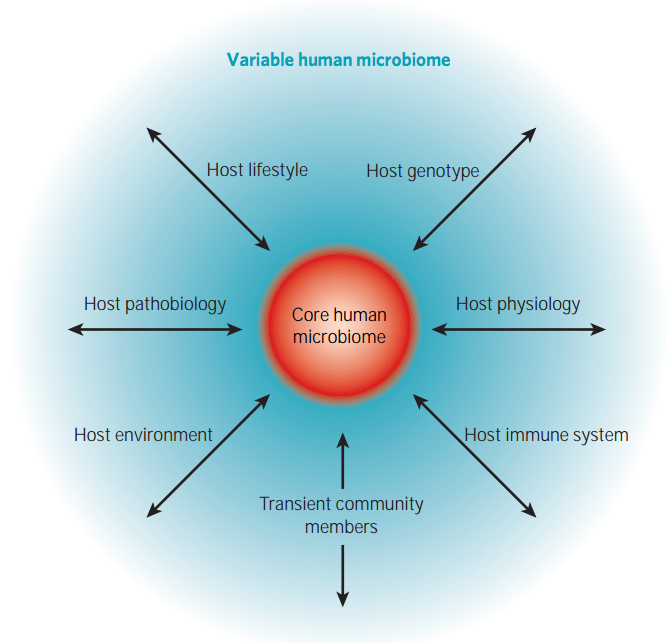
\includegraphics[width=\textwidth]{Figures/human_micro.png}
		\end{figure}
	\end{minipage}
	\footnotetext[2]{Peter J Turnbaugh et al. \textit{“The Human Microbiome Project.”}, Nature, 2007\\}
	%\autocite*{Turnbaugh2007}
}

\frame{
	\frametitle{RNApyro}
\begin{itemize}	\Large 
	\item Pseudo-energy composed of
		\begin{itemize}\large
			\item Stacked base pairs
			\item Isostericity through evolutionary information
		\end{itemize}
		\item Efficiently explore $m-$mutants space to generate nucleotides probabilities
	\end{itemize}
}

\frame{
	\frametitle{Additive Stacking-Pairs Energy \ES}
		\begin{itemize}
			\item Experimentally determined for every stacked canonical base pairs  						between $-3.5$ and $+1$
			\item For non canonical base pairs parameter $\beta$ which can be 
					$+\infty$ 					
		\end{itemize}	
		
%		\begin{minipage}{0.45\textwidth}
		
		\definecolor{mycolor1}{RGB}{244,14,77}
		\definecolor{mycolor2}{RGB}{57,181,74}
		\definecolor{mycolor3}{RGB}{46,49,146}
		\definecolor{mycolor4}{RGB}{151,113,43}
%		
%			\begin{tabular}{c}
%			\large
%				Energy\\ \\
%				\scalebox{1.3}{\textcolor{mycolor1}{A$=-1.3$}}\\\pause
%				\scalebox{1.3}{\textcolor{mycolor2}{B$=-1.5$}}\\\pause
%				\scalebox{1.3}{\textcolor{mycolor3}{C$=-2.1$}}\\\pause
%				\scalebox{1.3}{\textcolor{mycolor4}{D$=\beta$}}\\\hline\\
%				\scalebox{1.3}{$\ES(s,S)=-4.9+\beta$}
%			\end{tabular}
%		\end{minipage}
%		\begin{minipage}{0.45\textwidth}
			\begin{figure}
				\centering
					\includegraphics<1>[width=0.7\textwidth]{Figures/hairpin_stack_0.jpg}
					\includegraphics<2>[width=0.7\textwidth]{Figures/hairpin_stack_1.jpg}
					\includegraphics<3>[width=0.7\textwidth]{Figures/hairpin_stack_2.jpg}
					\includegraphics<4>[width=0.7\textwidth]{Figures/hairpin_stack_3.jpg}
					\includegraphics<5>[width=0.7\textwidth]{Figures/hairpin_stack_4.jpg}

			\end{figure}
%		\end{minipage}
}

\frame{
	\frametitle{Isostericity}
		\begin{itemize}
			\item In fact, interactions between \textbf{any} pair of nucleotides 									\item Between $+0$ and $+10$ reflects geometrical discrepancy 
				\footnote{Jesse Stombaugh et al. \textit{“Frequency and isostericity of RNA base pairs.”}, Nucleic acids research, 2009}	%\footfullcite{Stombaugh2009}
			\item We only consider \texttt{cWW} orientation
			\item  $\displaystyle\EI(s,S,\Omega) =\frac{1}{|\Omega|} \sum_{\substack{(i,j)\in S \text{pairs}}}\EI^{\Omega}_{(i,j),s_i s_j}$
		\end{itemize}

		\begin{minipage}{0.45\textwidth}		
			\begin{figure}
				\centering
										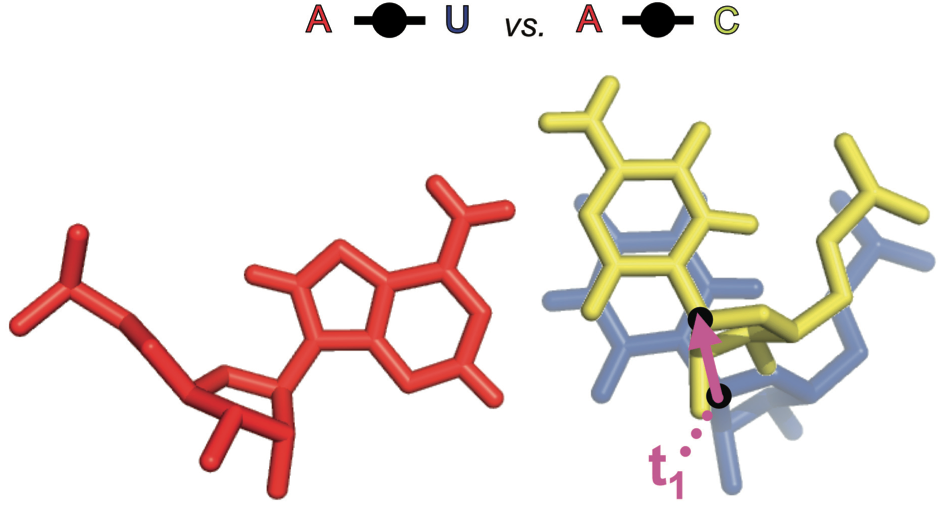
\includegraphics[width=\textwidth]{Figures/AU_AC_iso.png}\\
			\end{figure}
		\end{minipage}
		\begin{minipage}{0.45\textwidth}		
			\begin{table}
				\centering
				\begin{tabular}{cc}
								S							&		\texttt{...(...)...} \\
						s		& \texttt{...$\hspace{-7pt}\underbrace{\texttt{C}}_{i}\hspace{-7pt}$...$\hspace{-7pt}\underbrace{\texttt{A}}_{j}\hspace{-7pt}$...}\\
					\scalebox{1.2}{$\Omega$}			&	\\
					\texttt{...A...U...}	 &	 $+2.75$		\\
					\texttt{...G...U...} &	 $+4.76$			\\
					\texttt{...$\hspace{-7pt}\underbrace{\texttt{A}}_{s_i}\hspace{-7pt}$...$\hspace{-7pt}\underbrace{\texttt{U}}_{s_j}\hspace{-7pt}$...} &	 $+2.75$			\\\cline{2-2}
															 & $10.26/3$
				\end{tabular}
			\end{table}
		\end{minipage}


}


\frame{
	\frametitle{Probabilistic Model\\Sequence space}
	\begin{itemize}
		\item We can define a Boltzmann distribution
		\item Due to additive properties of the \texttt{Stacking Energy} and the
		\texttt{Isosteric Discrepancy} we can efficiently compute it with a 
			Dynamic Programming scheme
	\end{itemize}
	
%	\scalebox{1.3}{
	\begin{minipage}{0.45\textwidth}
		
		Boltzmann factor:\\ \scalebox{1.5}{$\qquad\mathcal{B}(s):= e^\frac{-\PE{s}}{RT}$}\vspace{7pt}\\
		Partition function:\vspace{7pt}\\\scalebox{1.5}{$\displaystyle\qquad\sum_s\mathcal{B}(s)$}\\\vspace{-15pt}
		\begin{align*}
			\PE{s}:&=\alpha\cdot\hspace{-20pt}\underbrace{\ES}_{\text{Stacking Energy}}\hspace{-15pt}(s,S)\\
			&+(1-\alpha)\cdot\hspace{-30pt}\underbrace{\EI}_{\text{Isosteric Discrepancy}}\hspace{-25pt}(s,S,\Omega)\\
		\end{align*}	
	\end{minipage}
	\begin{minipage}{0.45\textwidth}
	\begin{figure}
		\centering
		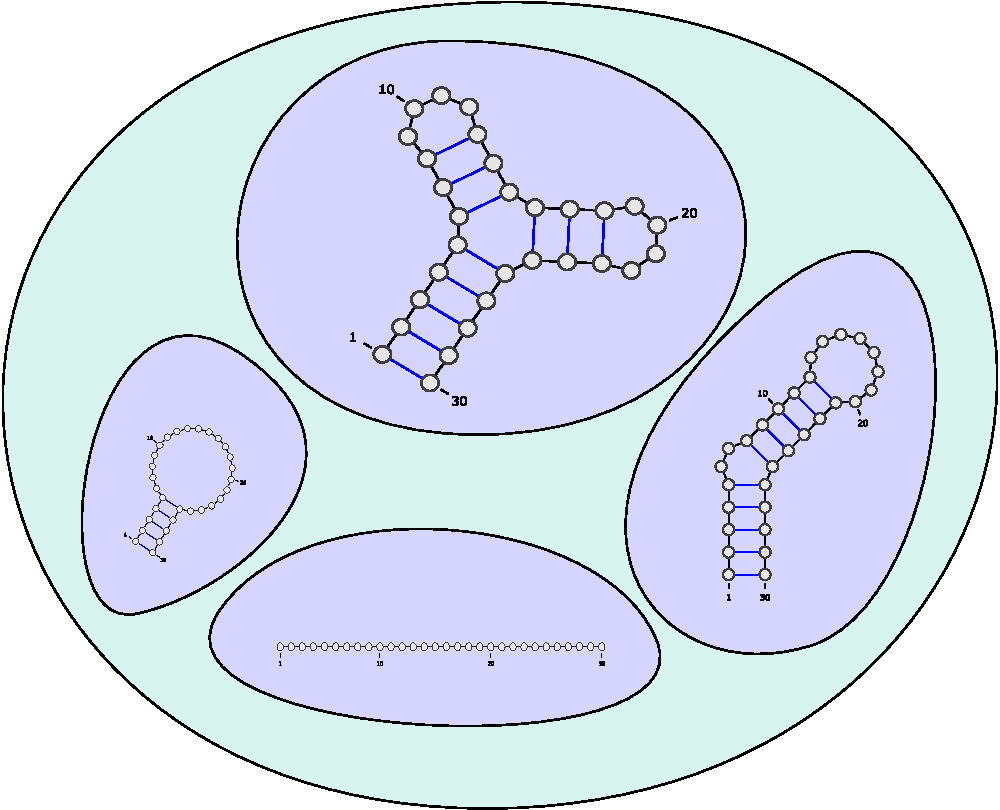
\includegraphics[width=1.2\textwidth]{Figures/convergence5.pdf}
	\end{figure}
	\end{minipage}

}

\frame{
	\frametitle{RNAPyro}
		Efficiently explore $m$ mutants space
	\vspace{-15pt}
	\begin{figure}
		\centering
		\resizebox{\textwidth}{!}{%!TEX root = ../vreinharz_RECOMB2013_talk.tex
\usetikzlibrary{shapes.multipart}

\newcommand{\SideEllRef}{15pt}
\newcommand{\TopEllRef}{15pt}
\newcommand{\BottomEllRef}{15pt}
\newcommand{\TopEll}{-20pt}

%\pgfdeclareimage[width=230pt,height=3em]{logo}{Figures/logo.png}
\pgfdeclareimage[width=0.5\textwidth]{boltz}{Figures/convergence_1}


\begin{tikzpicture}[every text node part/.style={align=center}]


\node[] (seq) at (0,0) {$\large \text{\texttt{UGGUUUC}}\cdots\text{\texttt{AACCCA}}$};

\coordinate (c-west) at ($ (seq.west) + (\SideEllRef,0) $);
\coordinate (c-east) at ($ (seq.east) - (\SideEllRef,0) $);
\coordinate (c-north) at ($ (seq.north) + (0,\TopEllRef) $);
\coordinate (c-south) at ($ (seq.south) - (0,\BottomEllRef) $);

\node[ellipse,fit=(c-west) (c-east) (c-north) (c-south),line width=2pt,color=black] (e0) {};
%\node[above=\TopEll of e0] {\Large no mutation};

\visible<3->{
\node[ellipse,fit=(e0),line width=2pt,color=black] (e1) {};
\node[above=\TopEll of e1] {\Large 1 mutation};
}

\visible<4->{
\node[ellipse,fit=(e1),line width=2pt,color=black] (e2) {};
\node[above=-25pt of e2.north] {\huge 2 mutations};
}

\visible<5->{
\node[ellipse,fit=(e2),line width=2pt,color=black] (e3) {};
\node[above=-37pt of e3.north] {\huge $m$ mutations\\\huge$\vdots$};
}

\begin{pgfonlayer}{background}
	\visible<5->{
	\node[ellipse,fit=(e2),draw, line width=2pt,color=black, fill=gray!50] {};
	}
	\visible<4->{
	\node[ellipse,fit=(e1),draw, line width=2pt,color=black, fill=gray!30] {};
	}
	\visible<3->{
	\node[ellipse,fit=(e0),draw, line width=2pt,color=black, fill=gray!10] {};
	}
	\node[ellipse,draw, fit=(c-west) (c-east) (c-north) (c-south),line width=2pt,color=black, fill=white] {};
\end{pgfonlayer}{background}



\coordinate (coord_boltz_fig) at ($ (e3.south east) + (200pt,100pt) $);


\node[right=10pt of coord_boltz_fig] (boltz_fig) {\pgfbox[right,top]{\pgfuseimage{boltz}}};


\node[above=20pt of e3] (MSE){\texttt{UGGUUU{\color{black}C}CUGCUUCA{\color{black}A}CAGUGC{\color{black}U}UGAACG{\color{black}G}AACCCA}\\
												\texttt{UGGGUU{\color{black}C}CUGCUUCA{\color{black}A}CAGUGC{\color{black}U}UGAAUG{\color{black}G}AACCCA}\\
												\texttt{GAGGUU{\color{black}C}UUGCUUCA{\color{black}G}CAGUGU{\color{black}U}UGGACG{\color{black}G}AACCUC}\\
												\texttt{CGGUUU{\color{black}C}CCGCUUCA{\color{black}A}CAGUGC{\color{black}U}UGGACG{\color{black}G}AAGCCG}\\
															\texttt{CCGAUU{\color{black}U}GUGCUUCA{\color{black}A}CAGUGA{\color{black}U}UGUACC{\color{black}G}AAACAG}};
\draw [line width=1.5pt,decoration={brace},decorate] (MSE.south west) -- (MSE.north west);
\node [left=10pt of MSE] {\scalebox{1.5}{$\text{\large MSE }(\Omega)$}};

\node[right=40pt of MSE] (rnapyro) {\Huge \color{red}\texttt{RNAPyro}};

\visible<2->{
\coordinate (arrow1) at ($ (rnapyro.south) - (40pt,0) $);
\path[->]<1-> (e0.east) edge [bend right=30,line width=2] (arrow1) ;
\coordinate (arrow5) at ($ (rnapyro.east) - (0,10pt) $);
\coordinate (arrow6) at ($ (boltz_fig) - (30pt,10pt) $);
\path[->]<1-> (arrow6) edge [bend right=15,line width=2,color=blue] node[above,sloped] {\color{black}\huge Stacking Energy} (arrow5) ;
\coordinate (arrow6) at ($ (rnapyro.north) + (0,10pt) $);
\path[->]<1-> (MSE.north) edge [bend left=55,line width=2,color=blue] node[above] {\color{black}\huge Isostericity} (arrow6);
}

\visible<3->{
\coordinate (arrow2) at ($ (rnapyro.south) - (20pt,0) $);
\path[->]<1-> (e1.east) edge [bend right=30,line width=2] (arrow2);
}

\visible<4->{
\coordinate (arrow3) at ($ (rnapyro.south) - (0pt,0) $);
\path[->]<1-> (e2.east) edge [bend right=22,line width=2] (arrow3);
}

\visible<5->{
\coordinate (arrow4) at ($ (rnapyro.south) + (20pt,0) $);
\path[->]<1-> (e3.east) edge [bend right=10,line width=2] (arrow4);
}


					
\end{tikzpicture}}
	\end{figure}
}

\frame{
	\frametitle{Computing probability}
	\vspace{-10pt}
	\scalebox{1.2}{$\text{Probability of } nt_9=x \text{ and } nt_{15} =y \text{ with }k\text{ mutations}$}
	\begin{figure}
		\centering
		\resizebox{1.1\textwidth}{!}{%!TEX root = ../vreinharz_RECOMB2013_talk.tex
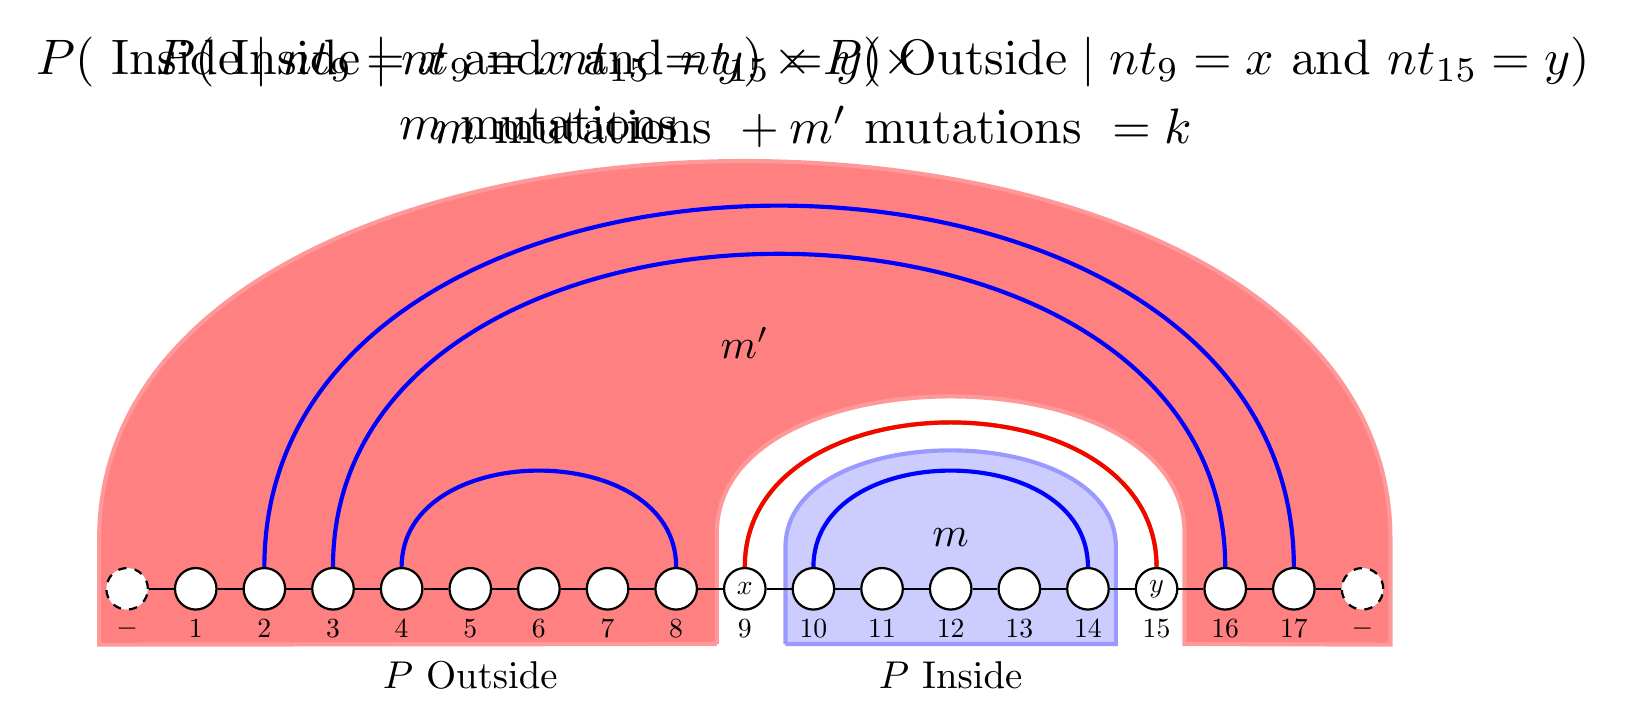
\begin{tikzpicture}

 \newcommand{\BSep}{9pt}
 \newcommand{\HSep}{250pt}
  \tikzstyle{base}=[circle,draw,thick,inner sep=0,minimum width=15pt,fill=white]
  \tikzstyle{basesmall}=[circle,draw,thick,inner sep=0,minimum width=10pt,fill=white]
  \tikzstyle{basephantom}=[base,dashed]
  \tikzstyle{linez}=[draw,snake=coil, segment aspect=.2,%
line after snake=0pt, 
        segment length=10pt,thick]
  \tikzstyle{lined}=[linez,draw,snake=none,thick]
  \tikzstyle{line}=[linez,draw,snake=none,thick]
  \tikzstyle{bp}=[in=90,out=90,draw,line width=1.5pt,blue,looseness=1.2]
  \tikzstyle{redbp}=[in=90,out=90,draw,line width=1.5pt,red,looseness=1.2]
  \tikzstyle{greenbp}=[in=90,out=90,draw,line width=1.5pt,green,looseness=1.2]
  \tikzstyle{inblock}=[trapezium,trapezium angle=83, fill=blue!20, draw=blue!40,line width=1.5pt, inner sep=0]
   \tikzstyle{outblock}=[trapezium,trapezium angle=83, fill=red!50, draw=red!40,line width=1.5pt, inner sep=0]
  \tikzstyle{lbl}=[inner sep=0]
  \tikzstyle{arr}=[line width=1.3pt,->]
%
\node[basephantom] (a-0) at (0,0) {};
\node[lbl,below=3pt of a-0] (i-0) {$-$};


\foreach \i in {1,...,17}
{
	\pgfmathtruncatemacro\j{\i - 1}

	\ifthenelse{\not\(\i = 9\)}{
		\ifthenelse{\not\(\i = 15\)}{
			\node[right=\BSep of a-\j, base] (a-\i) {};
		}
		{	
			\node[right=\BSep of a-\j, base] (a-\i) {$y$};		
		}
	}
	{
	\node[right=\BSep of a-\j, base] (a-\i) {$x$};
	}
	\node[lbl,below=3pt of a-\i] (i-\i) {$\i$};
	\path[lined] (a-\j) -- (a-\i);
}

\node[right=\BSep of a-17, basephantom] (a-18) {};
\node[lbl,below=3pt of a-18] (i-18) {$-$};
\path[lined] (a-17) -- (a-18);

\draw[bp] (a-2) to (a-17);
\draw[bp] (a-3) to (a-16);
\draw[bp] (a-4) to (a-8);
\draw[bp] (a-10) to (a-14);

\alt<1>{\draw[greenbp] (a-9) to (a-15);}	
	{\draw[redbp] (a-9) to (a-15);}

\begin{pgfonlayer}{background}	
	\visible<2->{
	\coordinate (northr1) at ($ (a-12.north) + (0,5pt) $);
  \node[rectangle,inner sep=2pt,fit=(a-10.west) (northr1) (a-14.east) (i-10) (i-14)] (r1) {};
  \path[inblock]   (r1.south west) to  (r1.south east) to (r1.north east) 		to[out=90,in=90] (r1.north west) to (r1.south west) ;
  \node[below=-10pt of r1.north] (m1) {\scalebox{1.5}{$m$}};
  	\node[below=15pt of a-12] (inside) {\scalebox{1.4}{$\mathds{P}\text{ Inside}$}};
	}
	\visible<2>{
	  \node[above=170pt of a-6] (total) {\scalebox{1.8}{$\mathds{P}(\text{ Inside}\mid nt_9=x\text{ and }nt_{15}=y)\times$}};
	  \node[below=0pt of total] (nut) {\scalebox{1.8}{$m\text{ mutations}$}};
	}

\end{pgfonlayer}{background}

\begin{pgfonlayer}{background}
	\visible<3>{
	\coordinate (northr1) at ($ (a-12.north) + (0,10pt) $);
	\node[rectangle,inner sep=2pt,fit=(a-9.west) (northr1) (a-15.east) (i-9.south) (i-15.south)] (r1) {};
	\coordinate (northr2) at ($ (a-9.north) + (0,8pt) $);
	\node[rectangle,inner sep=2pt, fit=(a-0.west) (northr2) (a-18.east) (i-0.south) (i-18.south)] (r2) {};
\path[outblock] (r1.south west) to (r2.south west) to (r2.north west) to[out=90,in=90] (r2.north east) to (r2.south east) to (r1.south east) to (r1.north east) to[out=90,in=90] (r1.north west) to (r1.south west);
	  	\node[below=15pt of a-5] (outside) {\scalebox{1.4}{$\mathds{P}\text{ Outside}$}};
		  \node[below=-80pt of r2.north] (m2) {\scalebox{1.5}{$m'$}};
			\node[above=170pt of a-10] (total) {\scalebox{1.8}{$\mathds{P}(\text{ Inside}\mid nt_9=x	\text{ and }nt_{15}=y)\times\mathds{P}(\text{ Outside}\mid nt_9=x\text{ and }nt_{15}=y)$}};
			\node[below=0pt of total] (nut) {\scalebox{1.8}{$m\text{ mutations }+ m'\text{ mutations }=k$}};
	}
\end{pgfonlayer}{background}


\end{tikzpicture}}
	\end{figure}
}



\frame{
	\frametitle{Inside}
	\begin{figure}
		\centering
		\resizebox{\textwidth}{!}{%!TEX root = main_RECOMB.tex
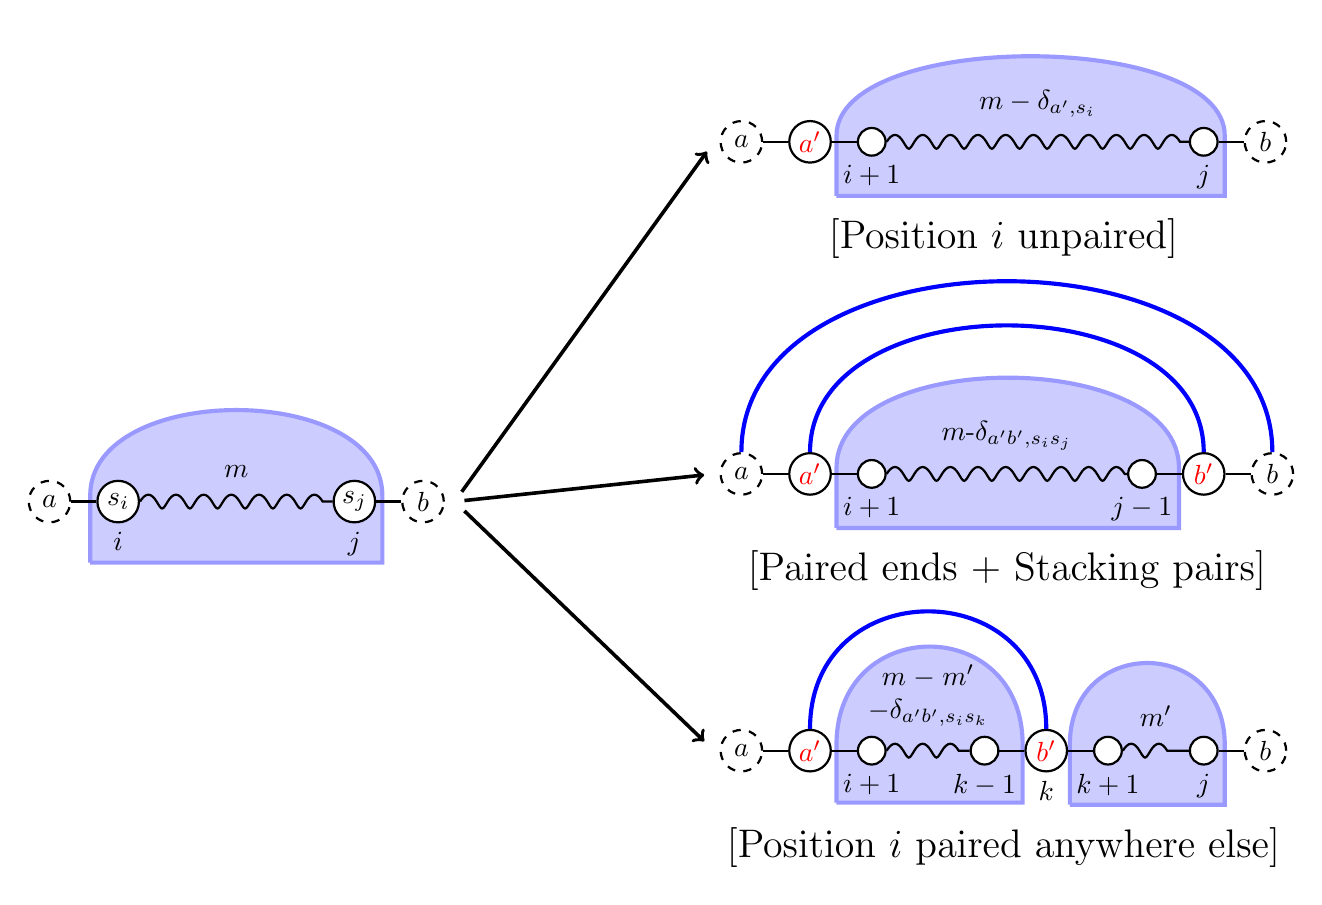
\begin{tikzpicture}

  \newcommand{\BSep}{9pt}
  \newcommand{\HSep}{250pt}
  \tikzstyle{base}=[circle,draw,thick,inner sep=0,minimum width=15pt,fill=white]
  \tikzstyle{basesmall}=[circle,draw,thick,inner sep=0,minimum width=10pt,fill=white]
  \tikzstyle{basephantom}=[base,dashed]
  \tikzstyle{linez}=[draw,snake=coil, segment aspect=.2,%
line after snake=0pt, 
        segment length=10pt,thick]
  \tikzstyle{lined}=[linez,draw,snake=none,thick]
  \tikzstyle{line}=[linez,draw,snake=none,thick]
  \tikzstyle{bp}=[in=90,out=90,draw,line width=1.5pt,blue,looseness=1.7]
  \tikzstyle{block}=[trapezium,trapezium angle=83, fill=blue!20, draw=blue!40,line width=1.5pt, inner sep=0]
  \tikzstyle{lbl}=[inner sep=0]
  \tikzstyle{arr}=[line width=1.3pt,->]

  \node[base] (a-1) at (0,0) {$s_i$};
  \node[base] (a-2) at (3,0) {$s_j$};
  \node[left=\BSep of a-1, basephantom] (a-0) {$a$};
  \node[right=\BSep of a-2, basephantom] (a-3) {$b$};
  \node[right=0 of a-3] (x) {};


  \path[linez] (a-1) --  node[pos=.5,above=5pt] (lbl1) {$m$}  (a-2);
  \path[lined] (a-0) -- (a-1);
  \path[lined] (a-2) -- (a-3);
  \node[lbl,below=3pt of a-1] (c1) {$i$};
  \node[lbl,below=3pt of a-2] (c2) {$j$};



  \begin{pgfonlayer}{background}
  \node[rectangle,inner sep=2pt,draw,fit=(a-1.west)(a-2.east) (c1) (c2)] (r1) {};
  \path[block]   (r1.south west) to  (r1.south east) to (r1.north east) to[out=90,in=90] (r1.north west) to (r1.south west) ;
  \end{pgfonlayer}{background}


\visible<2,5>{
\begin{scope}[xshift=\HSep,yshift=130pt]
  \node[base] (a-1) at (0,0) {\color{red}$a'$};
  \node[basesmall,right=\BSep of a-1] (a-1b)  {};
  \node[basesmall] (a-2) at (5,0) {};
  \node[left=\BSep of a-1, basephantom] (a-0) {$a$}; 
  \node[right=\BSep of a-2, basephantom] (a-3) {$b$};
  \path[linez] (a-1b) -- node[pos=.5,above=5pt] (lbl1) {$m-\delta_{a',s_i}$} (a-2);
  \path[line] (a-1) -- (a-1b);
  \path[lined] (a-0) -- (a-1);
  \path[lined] (a-2) -- (a-3);
  \node[below=3pt of a-1b, inner sep=0] (c1) {$i+1$};
  \node[below=3pt of a-2, inner sep=0] (c2) {$j$};

  \node[xshift=-2pt] at (a-0.west) (y1) {};

\begin{pgfonlayer}{background}
  \node[rectangle,inner sep=2pt,fit=(a-1b.west)(a-2.east) (c1) (c2)] (r1) {};
  \visible<2,5>{
  \path[block]   (r1.south west) to  (r1.south east) to (r1.north east) to[out=90,in=90,looseness=.7] (r1.north west) to (r1.south west) ;
  \path (a-0) to node[midway,yshift=-3.5em] {\relsize{+2}[Position $i$ unpaired]} (a-3);
	}
  \end{pgfonlayer}{background}

\end{scope}
\draw[arr] (x) -- (y1);
}

\visible<4->{
\begin{scope}[xshift=\HSep,yshift=-90pt]
  \node[base] (a-1) at (0,0) {\color{red}$a'$};
  \node[base] (a-p) at (3,0) {\color{red}$b'$};

  \node[basesmall,right=\BSep of a-1] (a-1b) {};
  \node[basesmall,left=\BSep of a-p] (a-pb)  {};
  \node[basesmall,right=\BSep of a-p] (a-pa)  {};

  \node[basesmall] (a-2) at (5,0) {};
  \node[left=\BSep of a-1, basephantom] (a-0) {$a$};
  \node[right=\BSep of a-2, basephantom] (a-3) {$b$};

  
  \path[linez] (a-1b) -- node[pos=.5,above=5pt,text width = 5em,text centered] (lbl1) {$m-m'$ $-\delta_{a'b',s_i s_k}$} (a-pb);
  \path[linez] (a-pa) -- node[pos=.5,above=5pt] (lbl2) {$m'$} (a-2);

  \path[line] (a-1) -- (a-1b);
  \path[line] (a-pb) -- (a-p);
  \path[line] (a-pa) -- (a-p);

  \path[lined] (a-0) -- (a-1);
  \path[lined] (a-2) -- (a-3);
  \node[lbl,below=3pt of a-1b] (c1) {$i+1$};
  \node[lbl,below=3pt of a-2] (c5){$j$};
  \node[lbl,below=3pt of a-p] (c3) {$k$};
  \node[lbl,below=3pt of a-pb] (c2){$k-1$};
  \node[lbl,below=3pt of a-pa] (c4){$k+1$};

  \draw[bp]  (a-1) to (a-p);
  \node[xshift=-2pt] at (a-0.west) (y2) {};

\begin{pgfonlayer}{background}
	\visible<4,5>{
  \node[rectangle,inner sep=2pt,fit=(a-1b.west)(a-pb.east) (c1) (c2)] (r1) {};
  \path[block]   (r1.south west) to (r1.south east) to (r1.north east) to[out=90,in=90,looseness=1.8] (r1.north west) to (r1.south west) ;

  \node[rectangle,inner sep=2pt,fit=(a-pa.west)(a-2.east) (c4) (c5)] (r2) {};
  \path[block]   (r2.south west) to (r2.south east) to (r2.north east) to[out=90,in=90,looseness=1.8] (r2.north west) to (r2.south west) ;

  \path (a-0) to node[midway,yshift=-3.5em] {\relsize{+2}[Position $i$ paired anywhere else]} (a-3);
  }
  \end{pgfonlayer}{background}

\end{scope}
\draw[arr] (x) -- (y2);
}


\visible<3,5>{
\begin{scope}[xshift=\HSep,yshift=10pt]
  \node[base] (a-1) at (0,0) {\color{red}$a'$};
  \node[base] (a-2) at (5,0) {\color{red}$b'$};

  \node[basesmall,right=\BSep of a-1] (a-1b) {};
  \node[basesmall,left=\BSep of a-2] (a-2b)  {};

  \node[left=\BSep of a-1, basephantom] (a-0) {$a$};
  \node[right=\BSep of a-2, basephantom] (a-3) {$b$};

  \path[linez] (a-1b) -- node[pos=.5,above=5pt] (lbl1) {$m$-$\delta_{a'b',s_is_j}$} (a-2b);

  \path[line] (a-1) -- (a-1b);
  \path[line] (a-2) -- (a-2b);
  \path[lined] (a-0) -- (a-1);
  \path[lined] (a-2) -- (a-3);
  \node[lbl,below=3pt of a-1b] (c1) {$i+1$};
  \node[lbl,below=3pt of a-2b] (c2){$j-1$};

  \draw[bp,looseness=1.1]  (a-1) to (a-2);
  \draw[bp,looseness=1.1]  (a-0) to (a-3);
  \node[xshift=-2pt] at (a-0.west) (y3) {};



\begin{pgfonlayer}{background}
  \node[rectangle,inner sep=2pt,fit=(a-1b.west)(a-2b.east) (c1) (c2)] (r1) {};
  \visible<3,5->{
  \path[block]   (r1.south west) to  (r1.south east) to (r1.north east) to[out=90,in=90,looseness=.9] (r1.north west) to (r1.south west) ;
  \path (a-0) to node[midway,yshift=-3.5em] {\relsize{+2}[Paired ends + Stacking pairs]} (a-3);}
  \end{pgfonlayer}{background}

\end{scope}
\draw[arr] (x) -- (y3);
}

\end{tikzpicture}}
	\end{figure}
}

\frame{
	\frametitle{Inside example}
	\begin{figure}[b!]
		\centering
		\resizebox{\textwidth}{!}{%!TEX root = ../vreinharz_RECOMB2013_talk.tex
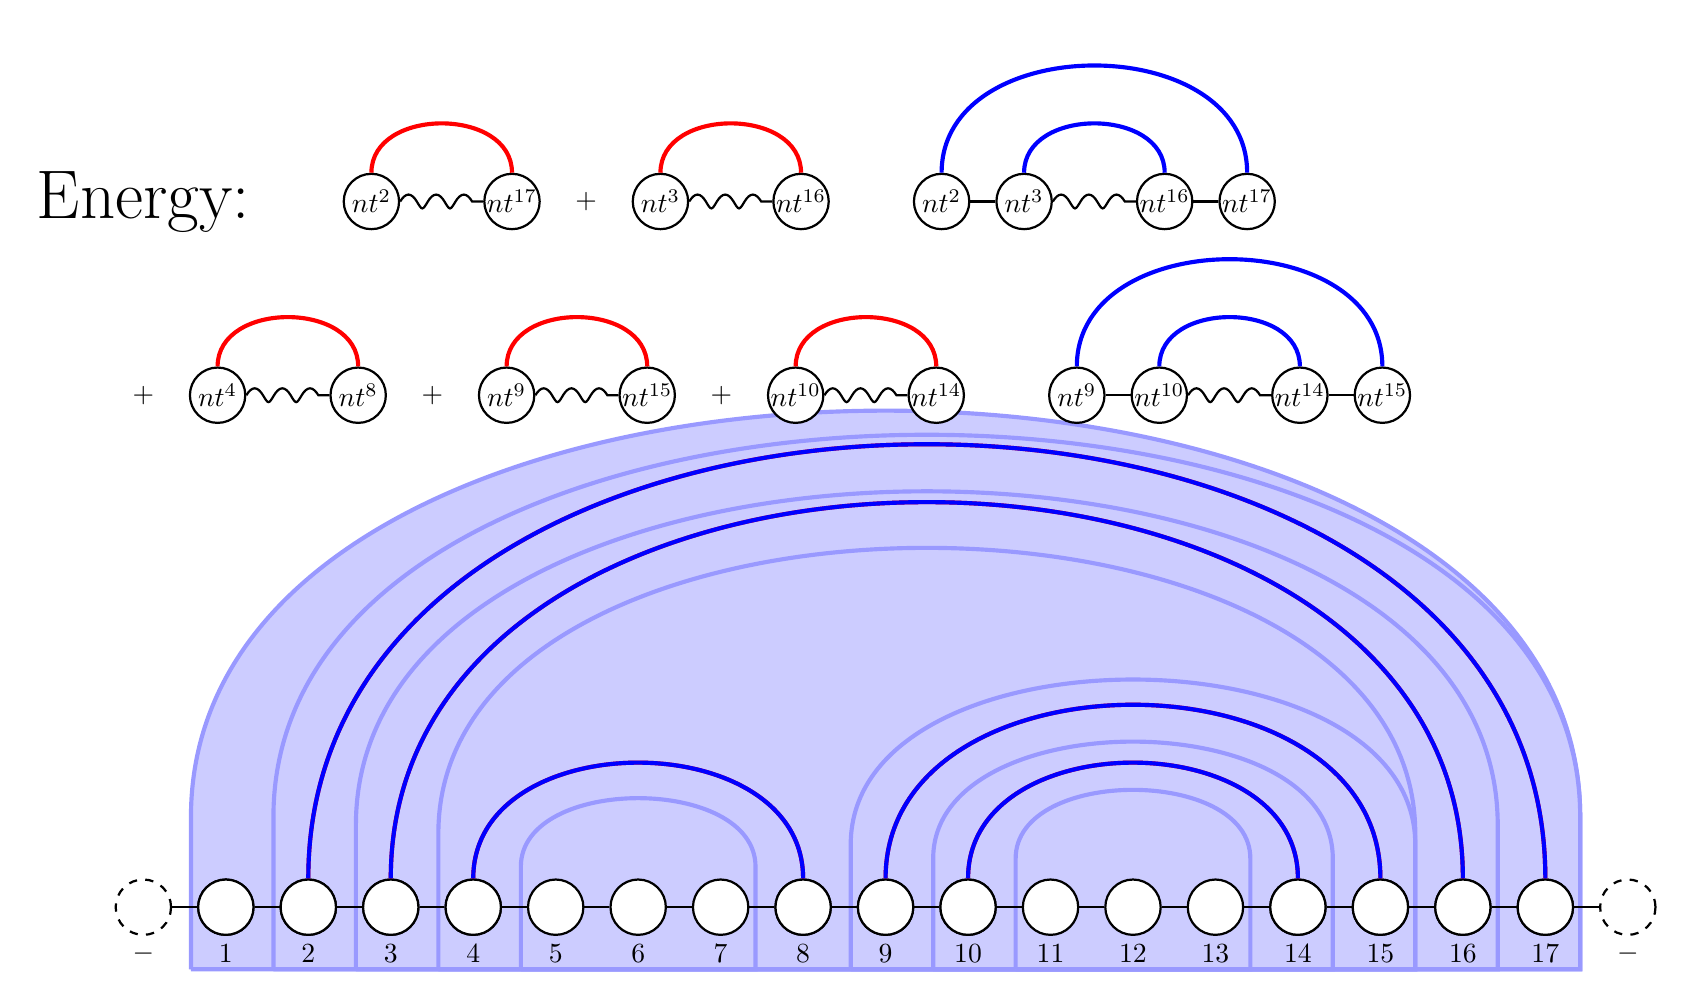
\begin{tikzpicture}

 \newcommand{\BSep}{9pt}
 \newcommand{\ESep}{30pt}
 \newcommand{\HSep}{250pt}
  \tikzstyle{base}=[circle,draw,thick,inner sep=0,minimum width=20pt,fill=white]
  \tikzstyle{basesmall}=[circle,draw,thick,inner sep=0,minimum width=10pt,fill=white]
  \tikzstyle{basephantom}=[base,dashed]
  \tikzstyle{linez}=[draw,snake=coil, segment aspect=.2,%
line after snake=0pt, 
        segment length=10pt,thick]
  \tikzstyle{lined}=[linez,draw,snake=none,thick]
  \tikzstyle{line}=[linez,draw,snake=none,thick]
  \tikzstyle{bp}=[in=90,out=90,draw,line width=1.5pt,blue,looseness=1.2]
  \tikzstyle{redbp}=[in=90,out=90,draw,line width=1.5pt,red,looseness=1.2]
  \tikzstyle{inblock}=[trapezium,trapezium angle=83, fill=blue!20, draw=blue!40,line width=1.5pt, inner sep=0]
   \tikzstyle{outblock}=[trapezium,trapezium angle=83, fill=red!50, draw=red!40,line width=1.5pt, inner sep=0]
  \tikzstyle{lbl}=[inner sep=0]
  \tikzstyle{arr}=[line width=1.3pt,->]
%

\begin{scope}[yshift=235pt]
  \node[] (tot) at (0,0) {\Huge Energy:};
	
	\visible<3->{
	\node[right=\ESep of tot, base] (iso-a-2) {$nt^2$};
	\node[right=\ESep of iso-a-2, base] (iso-a-17) {$nt^{17}$};
	\draw[redbp] (iso-a-2) to (iso-a-17);
	\path[linez] (iso-a-2) to (iso-a-17);
	}
	
	\visible<4->{
	\node[right=\BSep of iso-a-17] (p1) {$+$};
	
	\node[right=\BSep of p1, base] (iso-a-3) {$nt^3$};
	\node[right=\ESep of iso-a-3, base] (iso-a-16) {$nt^{16}$};
	\draw[redbp] (iso-a-3) to (iso-a-16);
	\path[linez] (iso-a-3) to (iso-a-16);
		
	
	\node[right=\ESep of iso-a-16,base] (e-a-2) {$nt^2$};
	\node[right=\BSep of e-a-2,base] (e-a-3) {$nt^3$};
	\node[right=\ESep of e-a-3,base] (e-a-16) {$nt^{16}$};
	\node[right=\BSep of e-a-16,base] (e-a-17) {$nt^{17}$};	
	\draw[bp] (e-a-2) to (e-a-17);
	\draw[bp] (e-a-3) to (e-a-16);
	\path[lined] (e-a-2) -- (e-a-3);
	\path[lined] (e-a-16) -- (e-a-17);
	\path[linez] (e-a-3) to (e-a-16);
	}
	
	\end{scope}

\begin{scope}[yshift=165pt]

	\visible<5->{
	\node[]  (p2) at (0,0) {$+$};
	
	\node[right=\BSep of p2,base] (iso-a-4) {$nt^4$};
	\node[right=\ESep of iso-a-4,base] (iso-a-8) {$nt^8$};
	\path[linez] (iso-a-4) to (iso-a-8);
	\draw[redbp] (iso-a-4) to (iso-a-8);
	}


	\visible<6->{
	\node[right=\BSep of iso-a-8] (p3) {$+$};

	\node[right=\BSep of p3,base] (iso-a-9) {$nt^9$};
	\node[right=\ESep of iso-a-9,base] (iso-a-15) {$nt^{15}$};
	\path[linez] (iso-a-9) to (iso-a-15);
	\draw[redbp] (iso-a-9) to (iso-a-15);
	}
	
	\visible<7->{
	\node[right=\BSep of iso-a-15] (p4) {$+$};
	
	\node[right=\BSep of p4,base] (iso-a-10) {$nt^{10}$};
	\node[right=\ESep of iso-a-10,base] (iso-a-14) {$nt^{14}$};
	\path[linez] (iso-a-10) to (iso-a-14);
	\draw[redbp] (iso-a-10) to (iso-a-14);

	\node[right=\ESep of iso-a-14,base] (e-a-9) {$nt^9$};
	\node[right=\BSep of e-a-9,base] (e-a-10) {$nt^{10}$};
	\node[right=\ESep of e-a-10,base] (e-a-14) {$nt^{14}$};
	\node[right=\BSep of e-a-14,base] (e-a-15) {$nt^{15}$};
	\path[lined] (e-a-9) to (e-a-10);
	\path[lined] (e-a-14) to (e-a-15);
	\path[linez] (e-a-10) to (e-a-14);
	\draw[bp] (e-a-9) to (e-a-15);
	\draw[bp] (e-a-10) to (e-a-14);
	}
\end{scope}

\begin{scope}[yshift=-20pt]
\node[basephantom] (a-0) at (0,0) {};
\node[lbl,below=3pt of a-0] (i-0) {$-$};

\alt<2>{\node[right=\BSep of a-0, base] (a-1) {\color{red}{$nt^1$}};}
	{\node[right=\BSep of a-0, base] (a-1) {};}

\alt<3>{\node[right=\BSep of a-1, base] (a-2) {\color{red}{$nt^2$}};}
	{\node[right=\BSep of a-1, base] (a-2) {};}
	
\alt<4>{\node[right=\BSep of a-2, base] (a-3) {\color{red}{$nt^3$}};}
	{\node[right=\BSep of a-2, base] (a-3) {};}
	
\alt<5>{\node[right=\BSep of a-3, base] (a-4) {\color{red}{$nt^4$}};}
	{\node[right=\BSep of a-3, base] (a-4) {};}

\node[right=\BSep of a-4, base] (a-5) {};
\node[right=\BSep of a-5, base] (a-6) {};
\node[right=\BSep of a-6, base] (a-7) {};


\alt<5>{\node[right=\BSep of a-7, base] (a-8) {\color{red}{$nt^8$}};}
	{\node[right=\BSep of a-7, base] (a-8) {};}
	
\alt<6>{\node[right=\BSep of a-8, base] (a-9) {\color{red}{$nt^9$}};}
	{\node[right=\BSep of a-8, base] (a-9) {};}
	
\alt<7>{\node[right=\BSep of a-9, base] (a-10) {\color{red}{$nt^{10}$}};}
	{\node[right=\BSep of a-9, base] (a-10) {};}	

\node[right=\BSep of a-10, base] (a-11) {};
\node[right=\BSep of a-11, base] (a-12) {};
\node[right=\BSep of a-12, base] (a-13) {};

\alt<7>{\node[right=\BSep of a-13, base] (a-14) {\color{red}{$nt^{14}$}};}
	{\node[right=\BSep of a-13, base] (a-14) {};}	
	
\alt<6>{\node[right=\BSep of a-14, base] (a-15) {\color{red}{$nt^{15}$}};}
	{\node[right=\BSep of a-14, base] (a-15) {};}	

\alt<4>{\node[right=\BSep of a-15, base] (a-16) {\color{red}{$nt^{16}$}};}
	{\node[right=\BSep of a-15, base] (a-16) {};}

\alt<3>{\node[right=\BSep of a-16, base] (a-17) {\color{red}{$nt^{17}$}};}
	{\node[right=\BSep of a-16, base] (a-17) {};}

\node[right=\BSep of a-17, basephantom] (a-18) {};


\foreach \i in {1,...,18}{
	\pgfmathtruncatemacro\j{\i - 1}
	\ifthenelse{\i<18}
	{\node[lbl,below=3pt of a-\i] (i-\i) {$\i$};}
	{\node[lbl,below=3pt of a-\i] (i-\i) {$-$};}
	\path[lined] (a-\j) -- (a-\i);
}


\alt<3>{\draw[redbp] (a-2) to (a-17);}
	{\draw[bp] (a-2) to (a-17);}
\alt<4>{\draw[redbp] (a-3) to (a-16);}
	{\draw[bp] (a-3) to (a-16);}
\alt<5>{\draw[redbp] (a-4) to (a-8);}
	{\draw[bp] (a-4) to (a-8);}
\alt<6>{\draw[redbp] (a-9) to (a-15);}
	{\draw[bp] (a-9) to (a-15);}
\alt<7>{\draw[redbp] (a-10) to (a-14);}
	{\draw[bp] (a-10) to (a-14);}

\begin{pgfonlayer}{background}	
	\visible<1>{
	\coordinate (northr1) at ($ (a-9.north) + (0,20pt) $);
  \node[rectangle,inner sep=2pt,fit=(a-1.west) (northr1) (a-17.east) (i-1) (i-17)] (r1) {};
  \path[inblock]   (r1.south west) to  (r1.south east) to (r1.north east) 		to[out=90,in=90] (r1.north west) to (r1.south west) ;
  }
\end{pgfonlayer}{background}

\begin{pgfonlayer}{background}	
	\visible<2>{
	\coordinate (northr1) at ($ (a-9.north) + (0,20pt) $);
  \node[rectangle,inner sep=2pt,fit=(a-2.west) (northr1) (a-17.east) (i-2) (i-17)] (r1) {};
  \path[inblock]   (r1.south west) to  (r1.south east) to (r1.north east) 		to[out=90,in=90] (r1.north west) to (r1.south west) ;
  }
\end{pgfonlayer}{background}

\begin{pgfonlayer}{background}	
	\visible<3>{
	\coordinate (northr1) at ($ (a-9.north) + (0,17pt) $);
  \node[rectangle,inner sep=2pt,fit=(a-3.west) (northr1) (a-16.east) (i-3) (i-16)] (r1) {};
  \path[inblock]   (r1.south west) to  (r1.south east) to (r1.north east) 		to[out=90,in=90] (r1.north west) to (r1.south west) ;
  }
\end{pgfonlayer}{background}

\begin{pgfonlayer}{background}	
	\visible<4>{
	\coordinate (northr1) at ($ (a-9.north) + (0,14pt) $);
  \node[rectangle,inner sep=2pt,fit=(a-4.west) (northr1) (a-15.east) (i-4) (i-15)] (r1) {};
  \path[inblock]   (r1.south west) to  (r1.south east) to (r1.north east) 		to[out=90,in=90] (r1.north west) to (r1.south west) ;
  }
\end{pgfonlayer}{background}

\begin{pgfonlayer}{background}	
	\visible<5>{
	\coordinate (northr1) at ($ (a-6.north) + (0,2pt) $);
  \node[rectangle,inner sep=2pt,fit=(a-5.west) (northr1) (a-7.east) (i-5) (i-7)] (r1) {};
  \path[inblock]   (r1.south west) to  (r1.south east) to (r1.north east) 		to[out=90,in=90] (r1.north west) to (r1.south west) ;
  }
\end{pgfonlayer}{background}

\begin{pgfonlayer}{background}	
	\visible<5>{
	\coordinate (northr1) at ($ (a-12.north) + (0,10pt) $);
  \node[rectangle,inner sep=2pt,fit=(a-9.west) (northr1) (a-15.east) (i-9) (i-15)] (r1) {};
  \path[inblock]   (r1.south west) to  (r1.south east) to (r1.north east) 		to[out=90,in=90] (r1.north west) to (r1.south west) ;
  }
\end{pgfonlayer}{background}

\begin{pgfonlayer}{background}	
	\visible<6>{
	\coordinate (northr1) at ($ (a-12.north) + (0,5pt) $);
  \node[rectangle,inner sep=2pt,fit=(a-10.west) (northr1) (a-14.east) (i-10) (i-14)] (r1) {};
  \path[inblock]   (r1.south west) to  (r1.south east) to (r1.north east) 		to[out=90,in=90] (r1.north west) to (r1.south west) ;
  }
\end{pgfonlayer}{background}

\begin{pgfonlayer}{background}	
	\visible<7>{
	\coordinate (northr1) at ($ (a-12.north) + (0,5pt) $);
  \node[rectangle,inner sep=2pt,fit=(a-11.west) (northr1) (a-13.east) (i-11) (i-13)] (r1) {};
  \path[inblock]   (r1.south west) to  (r1.south east) to (r1.north east) 		to[out=90,in=90] (r1.north west) to (r1.south west) ;
  }
\end{pgfonlayer}{background}

%\begin{pgfonlayer}{background}	
%	\coordinate (northr1) at ($ (a-9.north) + (0,20pt) $);
%  \node[rectangle,inner sep=2pt,fit=(a-1.west) (northr1) (a-17.east) (i-10) (i-14)] (r1) {};
%  \path[inblock]   (r1.south west) to  (r1.south east) to (r1.north east) 		to[out=90,in=90] (r1.north west) to (r1.south west) ;
%\end{pgfonlayer}{background}

\end{scope}


\end{tikzpicture}}
	\end{figure}
}


\frame{
	\frametitle{Outside}
	\begin{figure}
		\centering
		\resizebox{\textwidth}{!}{%!TEX root = main_RECOMB.tex

\begin{tikzpicture}
  \definecolor{rougeForb}{HTML}{eb23238f}
  \definecolor{rougeForbP}{HTML}{6d1515ff}

  \newcommand{\BSep}{9pt}
  \newcommand{\HSep}{400pt}
  \tikzstyle{base}=[circle,draw,thick,inner sep=0,minimum width=15pt,fill=white]
  \tikzstyle{basesmall}=[circle,draw,thick,inner sep=0,minimum width=10pt,fill=white]
  \tikzstyle{basephantom}=[base,dashed]
  \tikzstyle{linez}=[draw,snake=coil, segment aspect=.2,%
line after snake=0pt, 
        segment length=10pt,thick]
  \tikzstyle{lined}=[linez,draw,snake=none,thick]
  \tikzstyle{line}=[linez,draw,snake=none,thick]
  \tikzstyle{lineh}=[line,dashed]
  \tikzstyle{bp}=[in=90,out=90,draw,line width=1.5pt,blue,looseness=1.7]
  \tikzstyle{blockin}=[trapezium,trapezium angle=83, fill=blue!20, draw=blue!40,line width=1.5pt, inner sep=0]
  \tikzstyle{blockout}=[blockin,draw=red!50,fill=red!40]
  \tikzstyle{lbl}=[inner sep=0]
  \tikzstyle{arr}=[line width=1.3pt,->]

  \begin{scope}
  \node[basesmall] (n-beg) at (0,0) {};
  \node[base] (a-0) at (2,0) {$s_i$};
  \node[base] (a-3) at (6,0) {$s_j$};
  \node[basesmall] (n-end) at (8,0) {};
  \node[right=\BSep of a-0, basephantom] (a-1) {$a$};
  \node[left=\BSep of a-3, basephantom] (a-2) {$b$};
  \path[lineh] (a-1) --  node[pos=.5,above=40pt] (lbl1) {\relsize{+2}$m$}  (a-2);
  \path[lined] (a-0) -- (a-1);
  \path[lined] (a-2) -- (a-3);
  \path[linez] (n-beg) -- (a-0);
  \path[linez] (a-3) -- (n-end);

  \node[right=5pt of n-end] (x) {};


  \node[lbl,below=3pt of n-beg] (c0) {$0$};
  \node[lbl,below=3pt of a-0] (c1) {$i$};
  \node[lbl,below=3pt of a-3] (c2) {$j$};
  \node[lbl,below=3pt of n-end] (c3) {$n-1$};

  \begin{pgfonlayer}{background}
  \node[rectangle,inner sep=2pt,draw,fit=(n-beg)(a-0.east)(c1) (c0)] (r1) {};
  \node[rectangle,inner sep=2pt,draw,fit=(n-end)(a-3.west)(c2)(c3) ] (r2) {};
  \path[blockout]   (r1.south west) to (r1.south east) to (r1.north east) to[out=90,in=90,looseness=0.8] (r2.north west) to (r2.south west) to (r2.south east) to (r2.north east) to[out=90,in=90,looseness=0.8] (r1.north west) to (r1.south west) ;
  \end{pgfonlayer}{background}
  \end{scope}


\visible<2,6>{
  \begin{scope}[xshift=\HSep,yshift=170pt]
  \node[basesmall] (n-beg) at (0,0) {};
  \node[base] (a-0) at (2,0) {\color{red}$a'$};
  \node[basesmall,left=\BSep of a-0] (a-0b) {};
  \node[basesmall] (a-3) at (6,0) {};
  \node[basesmall] (n-end) at (8,0) {};
  \node[right=\BSep of a-0, basephantom] (a-1) {$a$};
  \node[left=\BSep of a-3, basephantom] (a-2) {$b$};
  \path[lineh] (a-1) --  node[pos=.5,above=40pt] (lbl1) {\relsize{+2}$m-\delta_{a',s_i}$}  (a-2);
  \path[lined] (a-0) -- (a-1);
  \path[lined] (a-2) -- (a-3);
  \path[lined] (a-0) -- (a-0b);
  \path[linez] (n-beg) -- (a-0b);
  \path[linez] (a-3) -- (n-end);

  \node[lbl,below=3pt of n-beg] (c0) {$0$};
  \node[lbl,below=3pt of a-0b] (c1) {$i-1$};
  \node[lbl,below=3pt of a-3] (c2) {$j$};
  \node[lbl,below=3pt of n-end] (c3) {$n-1$};

  \path (n-beg) to node[midway,yshift=-3em] {\relsize{+2}[Position $i$ unpaired]} (n-end);

  \node[left=5pt of n-beg] (y1) {};

  \begin{pgfonlayer}{background}
  \visible<2,6>{
  \node[rectangle,inner sep=2pt,draw,fit=(n-beg)(a-0b.east)(c1) (c0)] (r1) {};
  \node[rectangle,inner sep=2pt,draw,fit=(n-end)(a-3.west)(c2)(c3) ] (r2) {};
  \path[blockout]   (r1.south west) to (r1.south east) to (r1.north east) to[out=90,in=90,looseness=0.8] (r2.north west) to (r2.south west) to (r2.south east) to (r2.north east) to[out=90,in=90,looseness=0.8] (r1.north west) to (r1.south west) ;
  }
  \end{pgfonlayer}{background}
  \end{scope}
	\draw[arr] (x) -- (y1);
}	  
	
\visible<3,6>{  
  \begin{scope}[xshift=\HSep,yshift=60pt]
  \node[basesmall] (n-beg) at (0,0) {};
  \node[base] (a-0) at (2,0) {\color{red}$a'$};
  \node[basesmall,left=\BSep of a-0] (a-0b) {};
  \node[base] (a-3) at (6,0) {\color{red}$b'$};
  \node[basesmall,right=\BSep of a-3] (a-3b) {};
  \node[basesmall] (n-end) at (8,0) {};
  \node[right=\BSep of a-0, basephantom] (a-1) {$a$};
  \node[left=\BSep of a-3, basephantom] (a-2) {$b$};
  \path[lineh] (a-1) --  node[pos=.5,above=40pt] (lbl1) {\relsize{+2}$m-\delta_{a'b',s_is_j}$}  (a-2);
  \path[lined] (a-0) -- (a-1);
  \path[lined] (a-2) -- (a-3);
  \path[lined] (a-0) -- (a-0b);
  \path[lined] (a-3b) -- (a-3);
  \path[linez] (n-beg) -- (a-0b);
  \path[linez] (a-3b) -- (n-end);
  \draw[bp,looseness=.8] (a-1) to (a-2);
  \draw[bp,looseness=.8] (a-0) to (a-3);

  \node[lbl,below=3pt of n-beg] (c0) {$0$};
  \node[lbl,below=3pt of a-0b] (c1) {$i-1$};
  \node[lbl,below=3pt of a-3b] (c2) {$j+1$};
  \node[lbl,below=3pt of n-end] (c3) {$n-1$};

  \path (n-beg) to node[midway,yshift=-3em] {\relsize{+2}[Paired ends + Stacking pairs]} (n-end);


  \node[left=5pt of n-beg] (y2) {};

  \begin{pgfonlayer}{background}
  \visible<3,6>{
  \node[rectangle,inner sep=2pt,draw,fit=(n-beg)(a-0b.east)(c1) (c0)] (r1) {};
  \node[rectangle,inner sep=2pt,draw,fit=(n-end)(a-3b.west)(c2)(c3) ] (r2) {};
  \path[blockout]   (r1.south west) to (r1.south east) to (r1.north east) to[out=90,in=90,looseness=0.8] (r2.north west) to (r2.south west) to (r2.south east) to (r2.north east) to[out=90,in=90,looseness=0.8] (r1.north west) to (r1.south west) ;
  }
  \end{pgfonlayer}{background}
  \end{scope}
  \draw[arr] (x) -- (y2);
}

\visible<4,6>{
  \begin{scope}[xshift=\HSep,yshift=-50pt]
  \node[basesmall] (n-beg) at (0,0) {};
  \node[base] (a-0) at (1.8,0) {\color{red}$a'$};
  \node[basesmall,left=\BSep of a-0] (a-0b) {};
  \node[base] (a-3) at (6.25,0) {\color{red}$b'$};
  \node[basesmall] (b-1) at (4.0,0) {};
  \node[basesmall,left=\BSep of a-3] (b-2){};
  \node[basesmall,right=\BSep of a-3] (a-3b) {};
  \node[basesmall] (n-end) at (8,0) {};
  %\node[right=\BSep of a-0, basephantom] (a-1) {$a$};
  \node[left=\BSep of b-1, basephantom] (a-2) {$b$};
  \path[lineh] (a-0) --   (a-2);
  \path[lined] (a-2) -- (b-1);
  \path[linez] (b-1) -- node[pos=.5,above=8pt] (lbl1) {\relsize{+2}$m'$}  (b-2);
  \path (n-beg) -- node[pos=.5,above=40pt] (lbl1) {\relsize{+2}$m-\delta_{a'b',s_is_k}-m'$}  (n-end);
  \path[lined] (b-2) -- (a-3);
  \path[lined] (a-0) -- (a-0b);
  \path[lined] (a-3b) -- (a-3);
  \path[linez] (n-beg) -- (a-0b);
  \path[linez] (a-3b) -- (n-end);
  \draw[bp,looseness=.8] (a-0) to (a-3);
  \path (n-beg) to node[midway,yshift=-3em] {\relsize{+2}[Position $i$ paired to the right]} (n-end);

  \node[lbl,below=3pt of n-beg] (c0) {$0$};
  \node[lbl,below=3pt of a-0b] (c1) {$i-1$};
  \node[lbl,below=3pt of b-1] (c2) {$j$};
  \node[lbl,below=3pt of b-2] (c3) {$k-1$};
  \node[lbl,below=3pt of a-3] (c4) {$k$};
  \node[lbl,below=3pt of a-3b] (c5) {$k+1$};
  \node[lbl,below=3pt of n-end] (c6) {$n-1$};
  \node[left=5pt of n-beg] (y3) {};

  \begin{pgfonlayer}{background}
  \visible<4,6>{
  \node[rectangle,inner sep=2pt,draw,fit=(n-beg)(a-0b.east)(c1) (c0)] (r1) {};
  \node[rectangle,inner sep=2pt,draw,fit=(n-end)(a-3b.west)(c5)(c6) ] (r2) {};
  \path[blockout]   (r1.south west) to (r1.south east) to (r1.north east) to[out=90,in=90,looseness=0.8] (r2.north west) to (r2.south west) to (r2.south east) to (r2.north east) to[out=90,in=90,looseness=0.8] (r1.north west) to (r1.south west) ;

  \node[rectangle,inner sep=2pt,draw,fit=(b-1.west)(b-2.east) (c2) (c3)] (r3) {};
  \path[blockin]   (r3.south west) to (r3.south east) to (r3.north east) to[out=90,in=90,looseness=1.4] (r3.north west) to (r3.south west) ;
  }
  \end{pgfonlayer}{background}
  \end{scope}
  \draw[arr] (x) -- (y3);
}

\visible<5,6>{
  \begin{scope}[xshift=\HSep,yshift=-160pt]
  \node[basesmall] (n-beg) at (0,0) {};
  \node[base] (a-0) at (1.8,0) {\color{red}$b'$};
  \node[basesmall,left=\BSep of a-0] (a-0b) {};
  \node[base] (a-3) at (4.8,0) {\color{red}$a'$};
  \node[basesmall,right=\BSep of a-0] (b-1)  {};
  \node[basesmall,left=\BSep of a-3] (b-2){};
  \node[basesmall] (a-3b)  at (6.75,0) {};
  \node[basephantom,left=\BSep of a-3b] (a-3c){$b$};
  \node[basesmall] (n-end) at (8,0) {};
  \path (n-beg) to node[midway,yshift=-3em] {\relsize{+2}[Position $i$ paired to the left]} (n-end);


  %\node[right=\BSep of a-0, basephantom] (a-1) {$a$};
  %\node[left=\BSep of b-1, basephantom] (a-2) {$b$};
  \path[lined] (b-1) -- (a-0);
  \path[linez] (b-1) -- node[pos=.5,above=8pt] (lbl1) {\relsize{+2}$m'$}  (b-2);
  \path (n-beg) -- node[pos=.5,above=40pt] (lbl1) {\relsize{+2}$m-\delta_{a'b',s_is_k}-m'$}  (n-end);
  \path[lined] (a-3b) -- (a-3c);
  \path[lined] (a-0) -- (a-0b);
  \path[lined] (b-2) -- (a-3);
  \path[lineh] (a-3c) -- (a-3);
  \path[linez] (n-beg) -- (a-0b);
  \path[linez] (a-3b) -- (n-end);
  \draw[bp,looseness=1.05] (a-0) to (a-3);

  \node[lbl,below=3pt of n-beg] (c0) {$0$};
  \node[lbl,below=3pt of a-0b] (c1) {$k-1$};
  \node[lbl,below=3pt of a-0] (c2) {$k$};
  \node[lbl,below=3pt of b-1] (c3) {$k+1$};
  \node[lbl,below=3pt of b-2] (c4) {$i-1$};
  \node[lbl,below=3pt of a-3] (c5) {$i$};
  \node[lbl,below=3pt of a-3b] (c6) {$j$};
  \node[lbl,below=3pt of n-end] (c7) {$n-1$};
  \node[left=5pt of n-beg] (y4) {};

  \begin{pgfonlayer}{background}
  \visible<5,6>{
  \node[rectangle,inner sep=2pt,draw,fit=(n-beg)(a-0b.east)(c1) (c0)] (r1) {};
  \node[rectangle,inner sep=2pt,draw,fit=(n-end)(a-3b.west)(c6)(c7) ] (r2) {};
  \path[blockout]   (r1.south west) to (r1.south east) to (r1.north east) to[out=90,in=90,looseness=0.8] (r2.north west) to (r2.south west) to (r2.south east) to (r2.north east) to[out=90,in=90,looseness=0.8] (r1.north west) to (r1.south west) ;

  \node[rectangle,inner sep=2pt,draw,fit=(b-1.west)(b-2.east)  (c3) (c4)] (r3) {};
  \path[blockin]   (r3.south west) to (r3.south east) to (r3.north east) to[out=90,in=90,looseness=1.4] (r3.north west) to (r3.south west) ;
  \end{pgfonlayer}{background}
  }
  \end{scope}
  \draw[arr] (x) -- (y4);
}

\end{tikzpicture}}
	\end{figure}
}

\frame{
	\frametitle{Validation}
	\begin{itemize}
		\item Reconstruct 5s \texttt{rRNA} sequences 
%		\item Length $120$nt
		\item $45$ sequences without gap with less than $80\%$ of sequence similarity.
		\item $10\%$ random mutations
		\item Leave-one-out strategy
		\item Evaluate:
		\begin{itemize}
			\item Influence of $\alpha$ (i.e. weight of Stacking energy vs Isostericity)
			\item Over and under estimation of errors
			\item Confidence threshold
		\end{itemize}
	\end{itemize}
	\begin{figure}
		\centering
		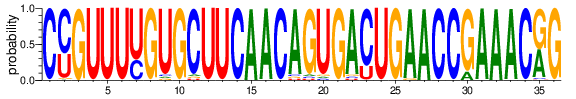
\includegraphics[width=0.8\textwidth]{Figures/logo.png}
	\end{figure}
}

\frame{
	\frametitle{Results}	
	\begin{figure}
			\centering
			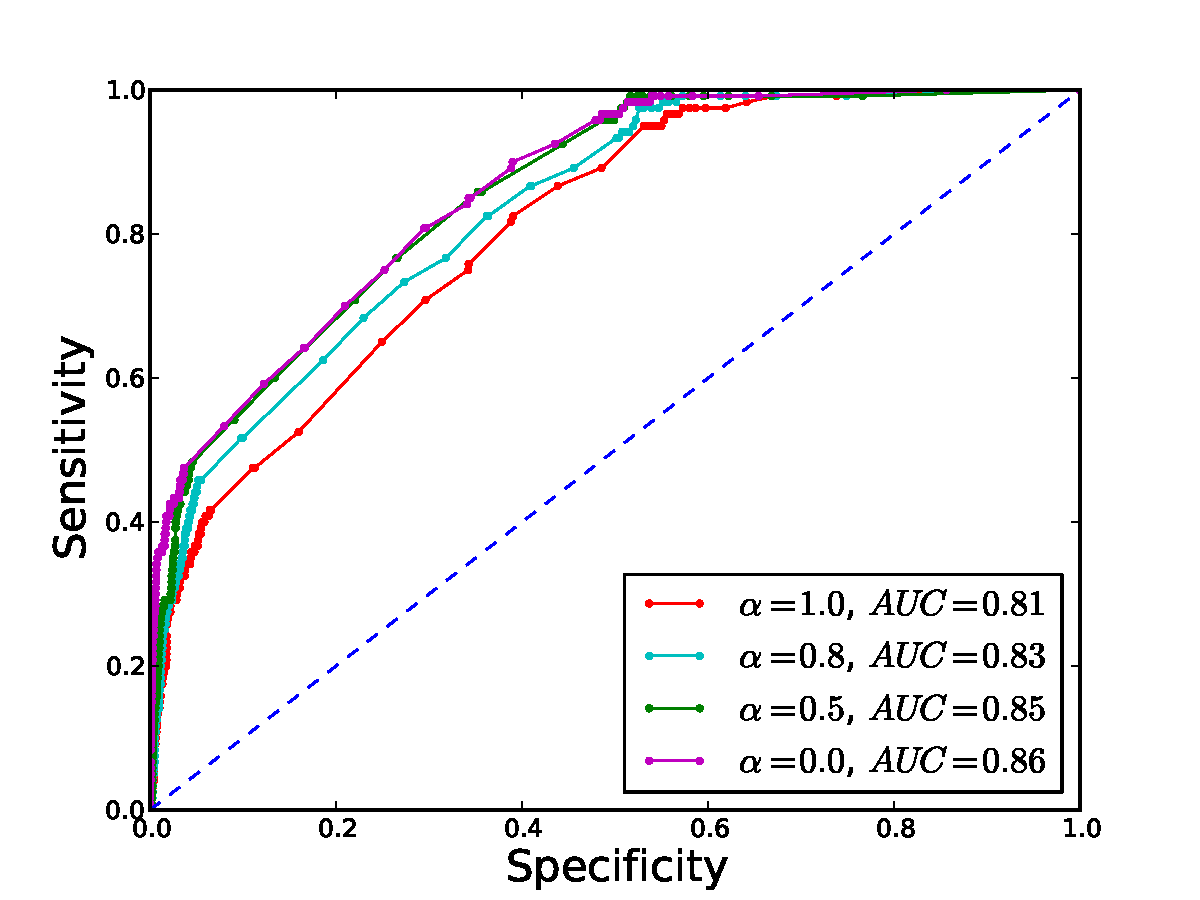
\includegraphics[height=0.75\textheight]{Figures/ROC_12.pdf}
		\end{figure}
	\begin{center}
		Correct number of mutations
	\end{center}
}

\frame{
	\frametitle{Results}
	\begin{minipage}{0.475\textwidth}
		\begin{figure}
			\centering
			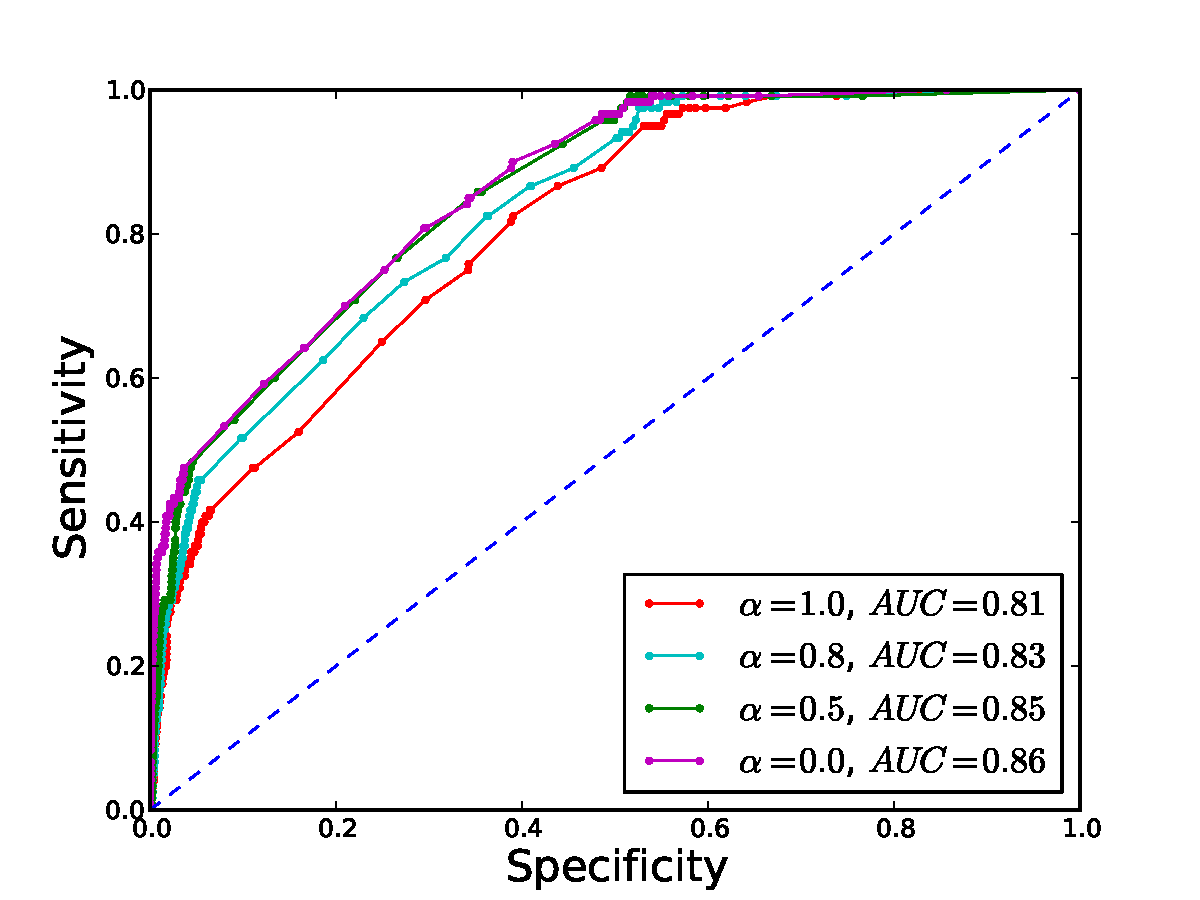
\includegraphics[width=1.1\textwidth]{Figures/ROC_12.pdf}
		\end{figure}
		Correct number of mutations
	\end{minipage}
	\begin{minipage}{0.475\textwidth}
		\begin{figure}
			\centering
			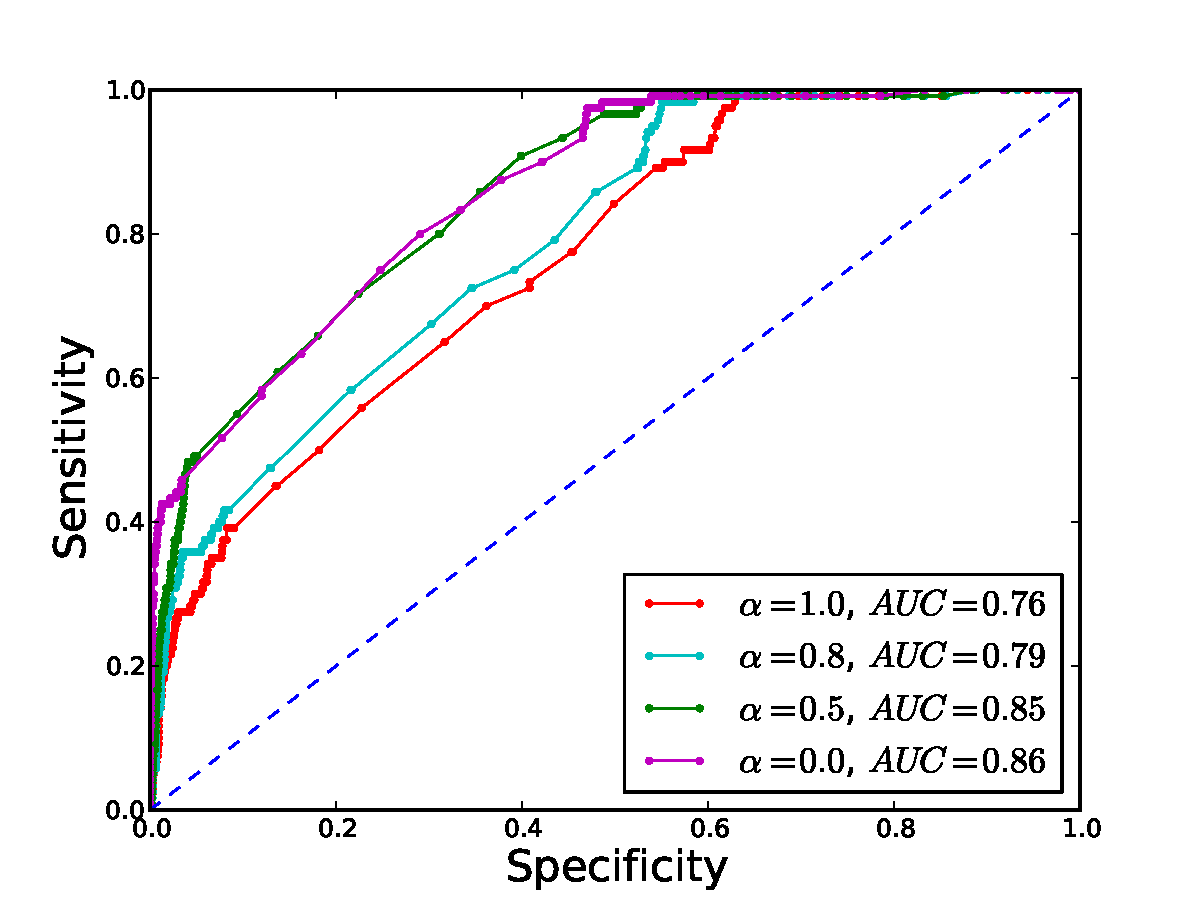
\includegraphics[width=1.1\textwidth]{Figures/ROC_24.pdf}
		\end{figure}
	Over estimation of mutations
	\end{minipage}
}


\frame{
	\frametitle{Future}
	\begin{minipage}{0.45\textwidth}
	\begin{itemize}
		\item Algorithmic
		\begin{itemize}
			\item Include gaps
			\item Implement full energetic model
		\end{itemize}
		\item Non-canonical annotations
		\item Incorporate into sequencing pipelines
	\end{itemize}
	\end{minipage}
	\begin{minipage}{0.45\textwidth}
		\begin{equation*}
		\label{eq:Z_rec}
		\resizebox{\textwidth}{!}{%
			$\Z{i,j}{m}{a,b}:=\left\{
	  \begin{array}{ll}
  		\displaystyle
      \sum_{\substack{a'\in \B,\\ \Kron_{a',s_i}\le m}}  
      \Z{i+1,j}{m-\Kron_{a',s_i}}{a',b} & \text{If }S_{i}=-1\\
      \displaystyle
      \sum_{\substack{a',b'\in \B^2,\\ \Kron_{a'b',s_is_j}\le m}}
			 e^{\frac{-E_{(i,j),ab \to a'b'}^{\Omega,\beta}}{RT}}
			 \cdot \Z{i+1,j-1}{m-\Kron_{a'b',s_is_j}}{a',b'}&
			 \text{Elif }S_i=j \land S_{i-1}=j+1\\
			 \displaystyle
      \sum_{\substack{a',b'\in \B^2,\\ \Kron_{a'b',s_is_k}\le m}}
      \sum_{m'=0}^{m-\Kron_{a'b',s_is_k}}
   		 e^{\frac{-E_{(i,k),\varnothing\to a'b'}^{\Omega,\beta}}{RT}}
      \cdot\Z{i+1,k-1}{m-\Kron_{a'b',s_is_k}-m'}{a',b'}
      \cdot\Z{k+1,j}{m'}{b',b} & \text{Elif }S_i=k \land i < k \leq j\\
      0 &\text{Otherwise}
		\end{array}\right.$}
		\end{equation*}
	\begin{equation*}
\resizebox{\textwidth}{!}{%
	$\Y{i,j}{m}{a,b} = \left\{
  \begin{array}{ll}
		\displaystyle
    \sum_{\substack{a'\in \B,\\ \Kron_{a',s_i}\le m}}
    \Y{i-1,j}{m- \Kron_{a',s_i}}{a',b} &
    \text{Elif }S_i=-1 \\
    \displaystyle
    \sum_{\substack{a'b'\in \B^2,\\ \Kron_{a'b',s_is_j}\le m}}
		 e^{\frac{-E_{(i,j),ab \to a'b'}^{\Omega,\beta}}{RT}}\cdot
    \Y{i-1,j+1}{m- \Kron_{a'b',s_is_j}}{a',b'} &
   	 \text{Elif }S_{i}=j \land S_{i+1}=j-1\\
		 \displaystyle
		 \sum_{\substack{a'b'\in \B^2,\\ \Kron_{a'b',s_is_k}\le m}}
		 \sum_{m'=0}^{m-\Kron_{a'b',s_is_k}}
  		 e^{\frac{-E_{(i,k),\varnothing\to a'b'}^{\Omega,\beta}}{RT}}
		 \cdot\Y{i-1,k+1}{m- \Kron_{a'b',s_is_k} - m'}{a',b'}
     \cdot\Z{j,k-1}{m'}{b,b'} &
		 \text{Elif }S_{i}=k \geq j\\
		 \displaystyle
		 \sum_{\substack{a'b'\in \B^2,\\ \Kron_{a'b',s_ks_i}\le m}}
		 \sum_{m'=0}^{m-\Kron_{a'b',s_ks_i}}
   	 e^{\frac{-E_{(k,i),\varnothing\to a'b'}^{\Omega,\beta}}{RT}}
		 \cdot\Y{k-1,j}{m- \Kron_{a'b',s_ks_i} - m'}{a',b}
     \cdot\Z{k+1,i-1}{m'}{a',b'} &
		 \text{Elif }-1 < S_{i}=k < i\\
		 0 & \text{Otherwise}
  \end{array}\right.$
	}
	\end{equation*}
	\begin{equation*}
\resizebox{\textwidth}{!}{%
$ \mathcal{W}^M_{\substack{i, [x]}} =  \left\{
	\begin{array}{ll}
			\sum_{m=0}^{M}
			\Y{i-1,i+1}{m-\Kron_{x,s_i}}{x,x}
		&\text{If }S_i = -1\\
			\displaystyle
			\sum_{m=0}^{M}
			\sum_{\substack{b\in B\\\Kron_{xb,s_is_k\leq m}}}
			\sum_{m'=0}^{m-\Kron_{xb,s_is_k}}
     	 e^{\frac{-E_{(i,k),\varnothing\to xb}^{\Omega,\beta} }{RT}}
			\cdot\Y{i-1,k+1}{m-\Kron_{xb,s_is_k-m'}}{x,b}
			\cdot\Z{i+1,k-1}{m'}{x,b}
		&\text{If }S_i=k>i\\
    \displaystyle
			\sum_{m=0}^{M}
			\sum_{\substack{b\in B\\\Kron_{bx,s_ks_i\leq m}}}
			\sum_{m'=0}^{m-\Kron_{bx,s_ks_i}}
     	 e^{\frac{-E^{\Omega, \beta}_{(k,i),\varnothing\to bx}}{RT}}
			\cdot\Y{k-1,i+1}{m-\Kron_{bx,s_ks_i-m'}}{b,x}
			\cdot\Z{k+1,i-1}{m'}{b,x}
		&\text{If }S_i=k<i
	\end{array}\right.
$}\label{eq:combine}
\end{equation*}
	\end{minipage}
}

\frame{
	\frametitle{Acknowledgment}
	\begin{minipage}{0.45\textwidth}
		\begin{itemize}
			\item Coauthors
			\begin{itemize}
				\item \JW
				\item \YP		
			\end{itemize}
		\item Discussions
			\begin{itemize}
				\item Rob Knight		
			\end{itemize}
		\end{itemize}	
	\begin{figure}
		\centering
		
\includegraphics[width=0.5\textwidth]{Figures/logofsm}
	\end{figure}
	\end{minipage}
	\begin{minipage}{0.45\textwidth}
		\begin{itemize}
			\item \texttt{ISCB} travel fellowship
		\end{itemize}
%			\item  French Agence Nationale de la Recherche (ANR) through the {\sc Magnum} {\tt ANR 2010 BLAN 0204} 
%project (to YP), 
%			\item FQRNT team grant 232983 (to VR and JW) 
%			\item NSERC Discovery grant 219671 (to JW).
%		\end{itemize}	
		\begin{minipage}{0.45\textwidth}
		\begin{figure}
			\centering
			
\includegraphics[width=\textwidth]{Figures/logoanr.png}
		\end{figure}
		\begin{figure}
				\centering
			
\includegraphics[width=\textwidth]{Figures/logoinria.png}
		\end{figure}
		\begin{figure}
			\centering
			
\includegraphics[width=\textwidth]{Figures/logofqrnt.png}
		\end{figure}
		\end{minipage}
		\begin{minipage}{0.45\textwidth}
		\begin{figure}
			\centering
			
\includegraphics[width=\textwidth]{Figures/logonserc}
		\end{figure}
		\begin{figure}
			\centering
			
\includegraphics[width=\textwidth]{Figures/logocnrs}
		\end{figure}
		\begin{figure}
			\centering
			
\includegraphics[width=\textwidth]{Figures/logo_X}
		\end{figure}
		\end{minipage}		
	\end{minipage}
}


\frame{
	\frametitle{RNAPyro}
	\begin{itemize}
		\item Efficient exploration of the mutant space
		\item Nt. probabilities in function of \texttt{Stacking Energy} and \texttt{Isostericity}
		\item Resilient to over estimation of errors
	\end{itemize}
		\begin{center}
		{\color{blue}\texttt{csb.cs.mcgill.ca}}
	\end{center}
	\begin{figure}
		\centering
		\resizebox{0.65\textwidth}{!}{%!TEX root = ../vreinharz_RECOMB2013_talk.tex
\usetikzlibrary{shapes.multipart}

\newcommand{\SideEllRef}{15pt}
\newcommand{\TopEllRef}{15pt}
\newcommand{\BottomEllRef}{15pt}
\newcommand{\TopEll}{-20pt}

%\pgfdeclareimage[width=230pt,height=3em]{logo}{Figures/logo.png}
\pgfdeclareimage[width=0.5\textwidth]{boltz}{Figures/convergence_1}


\begin{tikzpicture}[every text node part/.style={align=center}]


\node[] (seq) at (0,0) {$\large \text{\texttt{UGGUUUC}}\cdots\text{\texttt{AACCCA}}$};

\coordinate (c-west) at ($ (seq.west) + (\SideEllRef,0) $);
\coordinate (c-east) at ($ (seq.east) - (\SideEllRef,0) $);
\coordinate (c-north) at ($ (seq.north) + (0,\TopEllRef) $);
\coordinate (c-south) at ($ (seq.south) - (0,\BottomEllRef) $);

\node[ellipse,fit=(c-west) (c-east) (c-north) (c-south),line width=2pt,color=black] (e0) {};
%\node[above=\TopEll of e0] {\Large no mutation};

\node[ellipse,fit=(e0),line width=2pt,color=black] (e1) {};
\node[above=\TopEll of e1] {\Large 1 mutation};


\node[ellipse,fit=(e1),line width=2pt,color=black] (e2) {};
\node[above=-25pt of e2.north] {\huge 2 mutations};

\node[ellipse,fit=(e2),line width=2pt,color=black] (e3) {};
\node[above=-37pt of e3.north] {\huge $m$ mutations\\\huge$\vdots$};

\begin{pgfonlayer}{background}
	%\visible<5->{
	\node[ellipse,fit=(e2),draw, line width=2pt,color=black, fill=gray!50] {};
	%}
	%\visible<4->{
	\node[ellipse,fit=(e1),draw, line width=2pt,color=black, fill=gray!30] {};
	%}
	%\visible<3->{
	\node[ellipse,fit=(e0),draw, line width=2pt,color=black, fill=gray!10] {};
	%}
	\node[ellipse,draw, fit=(c-west) (c-east) (c-north) (c-south),line width=2pt,color=black, fill=white] {};
\end{pgfonlayer}{background}



\coordinate (coord_boltz_fig) at ($ (e3.south east) + (200pt,100pt) $);


\node[right=10pt of coord_boltz_fig] (boltz_fig) {\pgfbox[right,top]{\pgfuseimage{boltz}}};


\node[above=20pt of e3] (MSE){\texttt{UGGUUU{\color{black}C}CUGCUUCA{\color{black}A}CAGUGC{\color{black}U}UGAACG{\color{black}G}AACCCA}\\
												\texttt{UGGGUU{\color{black}C}CUGCUUCA{\color{black}A}CAGUGC{\color{black}U}UGAAUG{\color{black}G}AACCCA}\\
												\texttt{GAGGUU{\color{black}C}UUGCUUCA{\color{black}G}CAGUGU{\color{black}U}UGGACG{\color{black}G}AACCUC}\\
												\texttt{CGGUUU{\color{black}C}CCGCUUCA{\color{black}A}CAGUGC{\color{black}U}UGGACG{\color{black}G}AAGCCG}\\
															\texttt{CCGAUU{\color{black}U}GUGCUUCA{\color{black}A}CAGUGA{\color{black}U}UGUACC{\color{black}G}AAACAG}};
\draw [line width=1.5pt,decoration={brace},decorate] (MSE.south west) -- (MSE.north west);
\node [left=10pt of MSE] {\scalebox{1.5}{$\text{\large MSE }(\Omega)$}};

\node[right=40pt of MSE] (rnapyro) {\Huge \color{red}\texttt{RNAPyro}};

%\visible<2->{
\coordinate (arrow1) at ($ (rnapyro.south) - (40pt,0) $);
\path[->]<1-> (e0.east) edge [bend right=30,line width=2] (arrow1);
\coordinate (arrow5) at ($ (rnapyro.east) - (0,10pt) $);
\coordinate (arrow6) at ($ (boltz_fig) - (30pt,10pt) $);
\path[->]<1-> (arrow6) edge [bend right=15,line width=2,color=blue] node[above,sloped] {\color{black}\huge Stacking Energy}  (arrow5);
\coordinate (arrow6) at ($ (rnapyro.north) + (0,10pt) $);
\path[->]<1-> (MSE.north) edge [bend left=55,line width=2,color=blue] node[above,sloped] {\color{black}\huge Isostericity} (arrow6);
%}

%\visible<3->{
\coordinate (arrow2) at ($ (rnapyro.south) - (20pt,0) $);
\path[->]<1-> (e1.east) edge [bend right=30,line width=2] (arrow2);
%}

%\visible<4->{
\coordinate (arrow3) at ($ (rnapyro.south) - (0pt,0) $);
\path[->]<1-> (e2.east) edge [bend right=30,line width=2] (arrow3);
%}

%\visible<5->{
\coordinate (arrow4) at ($ (rnapyro.south) + (20pt,0) $);
\path[->]<1-> (e3.east) edge [bend right=15,line width=2] (arrow4);
%}


					
\end{tikzpicture}}
	\end{figure}
}

\end{document}



